%% OJAp submission, A&A class (aa.cls)
%% -------------------------------------------------------------------------

\documentclass{aa}

%% Core packages
\usepackage{graphicx}
\usepackage{amsmath,amssymb,amsfonts}
\usepackage{booktabs}
\usepackage{multirow}
\usepackage{xcolor}
%% <<CHANGED: removed \usepackage{natbib} — aa.cls loads it internally;
%%  duplicate load resets \bibpunct and breaks all citations>>
%% <<CHANGED: \bibliographystyle changed from sn-mathphys-num to plainnat>>
\usepackage{hyperref}      % optional but recommended for arXiv/OJAp
%% Changes made in this revision are marked with \rev{...} (bold red).
\newcommand{\rev}[1]{{\color{red}\textbf{#1}}}
\newcommand{\revm}[1]{{\color{red}\boldsymbol{#1}}}   % same, for use inside math

%% -------------------------------------------------------------------------
\begin{document}

   % first version: Sub-Snowline Formation of Gas-Giant Planets in Binary Systems
   \title{Gas-Giant Planets in Binary Systems Track the Tidal Truncation Radius of the Disc}

   \titlerunning{Gas giants in binaries track the truncation radius}

   \author{
     I. Kamai\inst{1}\corrauth{ilay.kamai@campus.technion.ac.il}%
       \thanks{These authors contributed equally to this work.}
     \and H.~B. Perets\inst{1,2}\email{hperets@physics.technion.ac.il}%
       \thanks{These authors contributed equally to this work.}
     \and J. Stegmann\inst{3}
     \and E. Grishin\inst{4,5}
   }

   \authorrunning{Kamai et al.}

   \institute{
     Physics Department, Technion -- Israel Institute of Technology,
       Haifa 32000, Israel
     \and
     ACRO, Open University of Israel, Ra'anana, Israel
     \and
     Max Planck Institute for Astrophysics,
       Karl-Schwarzschild-Str.\ 1, 85748 Garching, Germany
     \and
     School of Physics and Astronomy, Monash University,
       Clayton 3800, Australia
     \and
     OzGrav: ARC Centre of Excellence for Gravitational Wave Discovery,
       Clayton 3800, Australia
   }

   \date{Received \today}

%% -------------------------------------------------------------------------
%% aa.cls structured abstract: {Context}{Aims}{Methods}{Results}{Conclusions}
%% Context is optional (leave {} if not needed); Conclusions is optional.
%% -------------------------------------------------------------------------

   \abstract
   % Context
   {Gas-giant planets are thought to require conditions beyond the water
    snow line to build solid cores efficiently. In close binary star
    systems, the companion's gravity additionally limits the region of
    stable orbits, potentially excluding the zone where giants should form.}
   % Aims
   {We aim to identify binary systems in which gas giants exist despite
    the snow line lying in the dynamically unstable zone, and to \rev{test
    whether the size of the protoplanetary disc set by the companion
    determines their observed locations.}}
   % Methods
   {We analyse a catalogue of 811 circumstellar binary systems from
    \citet{Thebault2025}, identifying those hosting gas giants
    ($M_p \geq 0.15\,M_\mathrm{Jup}$) with snow lines larger than
    $0.8\,a_c$ as defined by \citet{Quarles_2020}. We compare their
    metallicity and eccentricity distributions with the background
    population, model snow-line evolution with \rev{MIST stellar tracks}, and fit a linear
    relation between observed planet semi-major axes and the tidal
    truncation radius from \citet{Pichardo2005}. \rev{We also run a
    one-dimensional gas--dust model of a tidally truncated circumprimary
    disc, with and without inflow from a circumbinary disc, to test
    whether the truncation edge hosts a dust trap.}}
   % Results
   {Among 393 gas-giant hosts, we identify 17 systems whose snow line
    lies in the dynamically unstable zone. Their metallicity and
    eccentricity distributions are consistent with the background
    population. \rev{The observed planet positions correlate with the
    truncation radius, $a_\mathrm{planet} = (0.57 \pm 0.05)\,r_t$
    (Pearson $r = 0.90$, $p = 10^{-3}$, intrinsic scatter 0.27\,dex),
    whereas gas giants with stable snow lines sit at
    $a_\mathrm{planet} \approx 0.08\,r_t$ with no correlation. The disc
    model produces no pressure maximum at the truncation edge, with or
    without inflow, and the dust-to-gas ratio there never exceeds 0.005:
    the edge does not trap solids in an axisymmetric disc with uniform
    viscosity, and delivered
    dust drifts through it.}}
   % Conclusions
   {\rev{Gas giants with unstable snow lines sit at a fixed fraction of
    the disc size set by the companion. This scaling, rather than a dust
    trap at the truncation edge, is the constraint that formation models
    for planets in close binaries must reproduce.}}

   \keywords{planet formation -- gas giants -- binary stars --
             protoplanetary discs}

   \maketitle

%% =========================================================================
\section{Introduction}
\label{sec:intro}
%% =========================================================================

Planetary formation is thought to be a bottom-up process
\citep{Safronov1972}, where dust particles accrete through aerodynamic
and gravitational collisions \citep{Dominik1997, Wada2009}. This
accretion is constrained by the gaseous protoplanetary disc lifetime
(approximately 3--10\,Myr; \citealt{Erc+17}) and the solids abundances.
For a gas giant to form, it is thought that a solid core exceeding a
critical mass (around 5--10\,$M_\oplus$) should form within the lifetime
of the gaseous disc, allowing a phase of runaway growth and accretion of
its massive gaseous envelope \citep{Greenberg1978, Pollack1996,
Armitage2024, Ikoma2025}. To rapidly reach the critical core mass, dust
aggregation must be highly efficient. An enhanced efficiency can result
from the sharp change in material properties of the disc around the snow
line, the distance to the host star at which the temperature is low
enough for water ice to form ($T_\mathrm{freeze} \approx 150$\,K). Ice
aggregation is approximately ten times more effective compared to typical
materials found below the snow line \citep{Blum2008, Gundlach2015},
suggesting the snow line as a critical lower limit for gas-giant
formation. However, here we identify observational evidence for
sub-snowline formation of gas giants in binaries \rev{and show that
their semi-major axes scale with the tidal truncation radius of the
disc, which is set by the binary orbit. We test whether the truncation
edge itself can concentrate solids and find that it cannot in an
axisymmetric disc with uniform viscosity, so the scaling is an empirical constraint on
formation models rather than evidence for a particular mechanism.}

When a planet is part of a binary system rather than a single star, the
gravitational tides raised by the stellar companion limit the region
where stable orbits exist. \citet{Holman1999} investigated the stability
of circumstellar orbiting planets in a binary system, and derived the
following relationship for the critical semi-major axis of an inner
(circumstellar) planet:
\begin{equation} \label{eq:stability}
  \frac{a_c}{a_b} = 0.464 - 0.380\mu - 0.631 e_b + 0.586\mu e_b
                    + 0.150 e_b^2 - 0.198 \mu e_b^2.
\end{equation}
Here, $a_c$ is the critical semi-major axis for stability,
$\mu = m_2/(m_1 + m_2)$ is the stellar mass ratio, with $m_2$ being the
companion mass and $m_1$ the primary mass, $e_b$ is the binary
eccentricity, and $a_b$ is the binary semi-major axis. This expression
was derived via least-squares fitting to N-body simulations, and is well
constrained near the centre of the parameter space; accuracy degrades at
extreme mass ratios or eccentricities. It also does not account for
mutual inclination $i$ between the binary and the planet orbit, which
can significantly change the stability boundary. As an improvement,
\citet{Quarles_2020} produced a numerical criterion that accounts for
$a_b, e_b, \mu$, and $i$; we use their tabulated values throughout this
work for all stability estimates.

Combining the snow-line and stability constraints, a gas giant in a
circumstellar system faces two simultaneous requirements: the snow line
$r_\mathrm{snow}$ defines a minimum formation distance, while $a_c$
defines a maximum. \rev{If $r_\mathrm{snow} > a_c$, core accretion
beyond the snow line is not available in situ. Such systems nevertheless
exist.} Analysing a catalogue of 811
circumstellar systems \citep{Thebault2025}, among which 393 host gas
giants, we found 17 gas giants where the snow line is larger than
$0.8\,a_c$ (we choose a conservative buffer of 0.8 to account for the
finite width of both boundaries; see Sect.~\ref{sec:methods}).
Figure~\ref{fig:all_systems} shows all 17 systems with their $a_c$ and
$r_\mathrm{snow}$.

\begin{figure*}
    \centering
    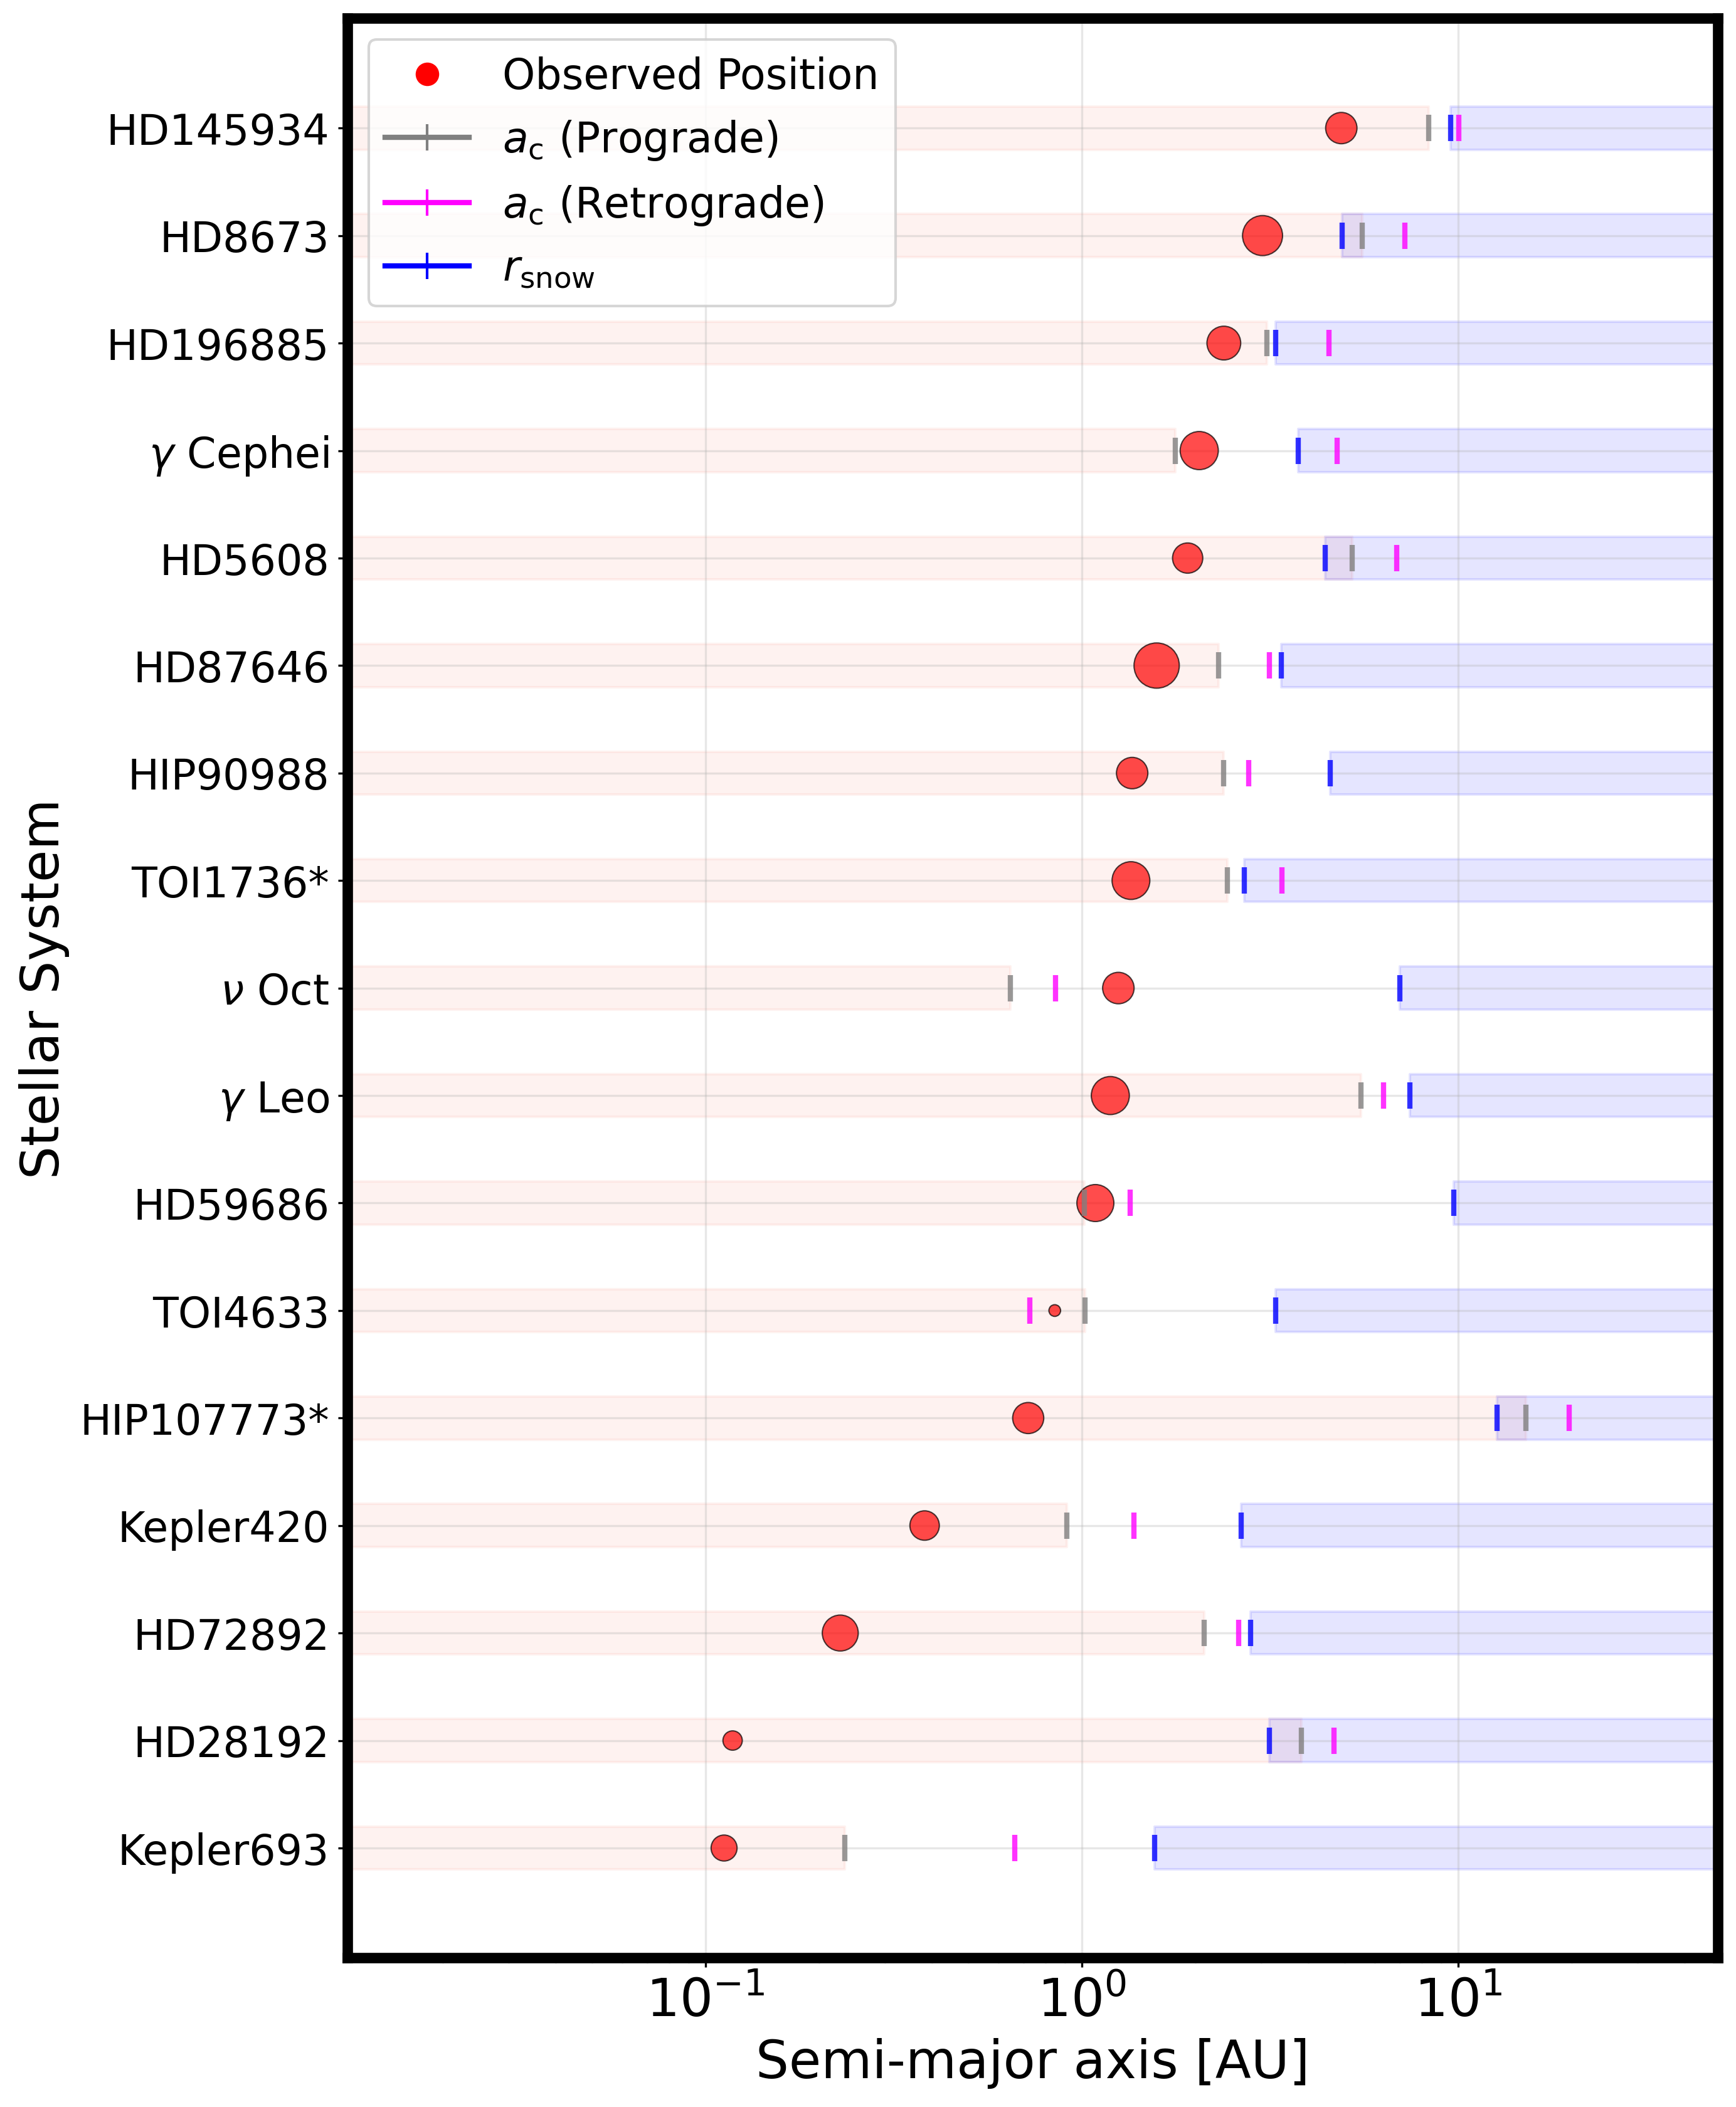
\includegraphics[width=\textwidth,height=0.85\textheight,keepaspectratio]{planetary_systems_plot.png}
    \caption{All circumstellar gas giants for which
    $r_\mathrm{snow} > 0.8\,a_c$ (prograde stability limits shown).
    The x-axis shows the current planetary semi-major axis. $a_c$ and
    $r_\mathrm{snow}$ are marked as grey and blue vertical lines
    (see Sect.~\ref{sec:methods} for calculation details). The pink
    shaded region marks the prograde-stable zone; the blue shaded region
    marks the ice-formation zone. Note that retrograde stability limits
    extend significantly further out, but the path to retrograde
    configurations is not well understood for these systems
    \citep{Stegmann2025}. Systems with an asterisk have no measured
    eccentricity; zero eccentricity is assumed for their stability
    calculation. \rev{Three systems lie beyond the prograde $a_c$:
    $\nu$~Oct ($a_\mathrm{planet}/a_c = 1.9$) and HD~59686 (1.07), both
    proposed to host retrograde or second-generation planets
    \citep{cheng_retrograde_2025, Ortiz2016}, and $\gamma$~Cephei (1.16),
    whose position is consistent with $a_c$ within the uncertainties in
    $\mu$, $e_b$, $a_b$ and the mutual inclination. Their inclusion does
    not affect the main conclusions.}}
    \label{fig:all_systems}
\end{figure*}

Finding such a sample of planets \rev{that standard theory does not
readily explain} has great potential to test our understanding of planet formation
processes, and in particular the formation of gas giants, and
potentially opens the door for new formation channels.

There might be several explanations for this apparent paradox.
In-situ sub-snowline formation of gas giants was suggested to be
potentially possible through (i)~\emph{Pebble accretion at inner
pressure traps} -- at the dead-zone inner edge, silicate sublimation
front, or magnetospheric cavity -- which can concentrate drifting solids
and accelerate core growth; this pathway predicts giants clustered at
relatively small radii, near 0.1--1\,AU for solar-type stars with
metal-enriched envelopes \citep{Lambrechts2012, Lambrechts2014,
Bitsch2015, Chatterjee2014}; (ii)~\emph{Reduced runaway thresholds via
envelope enrichment and low opacities}, which allow gas accretion at
smaller core masses, favouring metal-rich hosts \citep{HoriIkoma2011,
VenturiniHelled2017}; and (iii)~\emph{Local assembly by mergers of
migrating super-Earth cores}, which can push a merged core over the
runaway limit interior to the snow line \citep{HansenMurray2013,
Boley2016}. However, most of our identified planets are at larger
separations than these models suggest (see Fig.~\ref{fig:all_systems}),
and their metallicities are consistent with the background population
(see Fig.~\ref{fig:feh_e_hists}).

Another straightforward possibility is that the snow line evolves with
stellar luminosity and was located in a stable region at the onset of
planet formation. To test this, for each unstable giant we examined the
luminosity of a young single star with the same metallicity and mass,
\rev{using MIST stellar evolution tracks \citep[built with MESA;][]{Choi2016,
Paxton2011, Jermyn2023}.} Out of 13 systems with
measured metallicities and masses, only four had a stable snow line at
formation time (around 2\,Myr; see Fig.~\ref{fig:snowline_evolution}).
While this evolutionary scenario may be physically valid for those four
individual cases, it is insufficient as a general explanation for two
reasons. First, it fails for the remaining systems, whose snow line is
dynamically unstable even at the earliest stellar ages. Second, and more
critically, the snowline-evolution scenario is purely qualitative: it
can address \emph{whether} a giant could have formed, but not
\emph{where} --- it provides no prediction for the specific observed
semi-major axis, which \rev{the empirical relation with the truncation
radius (Sect.~\ref{sec:results}) does}.
A further possibility is that the planet formed before the binary
assembled. This scenario is unlikely, as the timescale for binaries to
form at wider separations and migrate inwards is usually much shorter
than the disc lifetime \citep[e.g.][]{Generozov2025}. Capture from a
different system through an exchange interaction would predict a
significant difference in eccentricity between this population and the
general gas-giant population; no such difference is seen
(Fig.~\ref{fig:feh_e_hists}), making this unlikely, though statistics
are small. \citet{Gong2018} investigated the capture of a circumbinary
planet into a close circumstellar orbit, but this probability decreases
dramatically for small binary separations, high eccentricities, or high
mass ratios, and cannot explain the general sample.

\rev{Planet formation in close binaries has been studied extensively.
Planetesimal accretion is hampered by the collision velocities excited by
the companion \citep{Thebault2006, Paardekooper2008} unless the gravity
of the gas disc damps the excitation \citep{Rafikov2013, Silsbee2015,
Silsbee2021}. Hydrodynamical models of $\gamma$~Cephei-like circumprimary
discs \citep{Kley2008, Muller2012, Jordan2021, Marzari2025b} find
truncation at a few au, modest disc eccentricity, and short disc
lifetimes without an external gas supply. Dust drifts inward faster in
truncated discs, and dust discs in binaries are observed to be smaller
than the truncation radius \citep{Zagaria2021, Zagaria2021b}. Most
recently, global pebble-accretion models find that truncation suppresses
in-situ growth of S-type planets for binary separations below
$\sim160$\,au \citep{Venturini2026}, unless the circumprimary disc is
replenished from a circumbinary reservoir, in which case giants can form
in $\gamma$~Cephei-like systems \citep{Ronco2026}. The sample presented
here is the observational counterpart of that tension: these giants
exist, and we ask where in the disc they formed.}

\rev{We show that their locations follow the tidal truncation radius of
the disc, test one candidate explanation, that the truncation edge itself
concentrates the solids they formed from, and find that it does not,
leaving the scaling as the empirical constraint any formation channel
for these planets must satisfy.}

%% =========================================================================
\section{Methods}
\label{sec:methods}
%% =========================================================================

\subsection{Sample selection}
\label{sec:sample}

We estimate the water-ice snow line for each system in the catalogue.
We assume an irradiated disc where the temperature profile is
\begin{align}
    \frac{T(r)}{T_\odot(1 \, \text{AU})} =
    \left(\frac{L}{L_\odot}\right)^{\frac{1}{4}}
    \left(\frac{r}{1 \, \text{AU}}\right)^{-\frac{1}{2}},
\end{align}
\rev{with $T_\odot(1\,\mathrm{AU}) = 280$\,K \citep{Hayashi1981},}
which, when evaluated at the water-ice condensation temperature
(\rev{$T_\mathrm{freeze} \approx 170$\,K; \citealt{Hayashi1981,
Sasselov2000}}), gives the snow-line distance as
\begin{align}
    r_{\rm snow} \approx 2.7 \left(\frac{L}{L_\odot}\right)^{\frac{1}{2}}
    \, \text{AU}.
\end{align}
This result is consistent with the positions of gas giants in our solar
system. \rev{Condensation temperatures of 120--170\,K are quoted in
the literature \citep{Oberg2011, Sasselov2000}; since
$r_\mathrm{snow} \propto T_\mathrm{freeze}^{-2}$, the lower values place
the snow line up to a factor of two further out, which would add systems
to the unstable sample but remove none of the 17, so the selection is
conservative in that direction. A temperature 10\% above 170\,K moves the
snow line 17\% inward and would drop the four systems closest to the
threshold (HD~28192, HIP~107773, HD~5608 and HD~8673), two of them from
the fit sample of Sect.~\ref{sec:results}; the slope with the remaining
seven is 0.63 ($r = 0.89$, $p = 7\times10^{-3}$).} We treat the snow line here as the water-ice
boundary; other molecular species (CO, HCN) condense at lower
temperatures further out and are not relevant to the present analysis.

We calculated the critical distance for stability, $a_c$, using the
tables from \citet{Quarles_2020}, which provide stability values for
different values of $\mu$, $e_b$, and $i$. We interpolated between
tabulated values and extrapolated for values outside the table boundary
($e_b > 0.8$, for example). \rev{Three gas-giant hosts have $e_b > 0.8$
($\gamma$~Leo, 0.84; $\tau$~Boo, 0.87; TOI~4633, 0.91), so their $a_c$ is
extrapolated. Since $a_c$ enters only through the selection of unstable
gas giants, defined below as $r_\mathrm{snow} \geq 0.8\,a_c$, this
matters only if it could move a system across that threshold: the snow
lines of TOI~4633 and $\gamma$~Leo lie at $3.2\,a_c$ and $1.35\,a_c$, so both
remain unstable for any plausible $a_c$, while $\tau$~Boo is marginal
and is excluded on other grounds (below). The fit of Sect.~\ref{sec:results}
uses $r_t$, not $a_c$; dropping TOI~4633, the only one of the three in
the fit sample, changes the slope from 0.569 to 0.565.} We note that the \citet{Quarles_2020}
criterion is based on test-particle N-body simulations and does not
account for the gravitational influence of the gaseous disc on stability
limits or for the finite planetary mass; these represent inherent
limitations that should be borne in mind when interpreting individual
systems. We adopt coplanar ($i = 0$) orbits for systems without measured
inclinations. \rev{Only four of the 17 unstable systems have a catalogued
mutual inclination (Kepler~693, Kepler~420, $\gamma$~Cephei and HD~196885).
In the \citet{Quarles_2020} tables an inclination of $45^\circ$ halves
$a_c$ relative to the coplanar value for every system in our fit sample,
so the coplanar assumption is conservative: a misaligned system is more,
not less, likely to have its snow line in the unstable zone.}

We define a gas giant as a planet with $M_p \geq 0.15\,M_\mathrm{Jup}$
(approximately $0.5\,M_\mathrm{Saturn}$) and an `unstable gas giant'
as a gas giant with $r_\mathrm{snow} \geq 0.8\,a_c$. We note that
this threshold includes sub-Saturn-mass planets that may have radii of
only 3--4\,$R_\oplus$. These objects still require a gaseous envelope
constituting a significant fraction of their total mass, and therefore
still require a sufficiently massive solid core to trigger runaway gas
accretion \citep{Pollack1996}; the snow-line constraint on core growth
applies equally to them. \rev{The relation between planet position and
disc size derived below does not depend on the final planetary mass.} The factor of 0.8 accounts for the
fact that both $a_c$ and $r_\mathrm{snow}$ represent approximate
boundaries with finite width; varying it to 0.7 or 0.9 yields 19 or
13 systems respectively, without changing the overall results or
conclusions. Out of 811 systems in the catalogue, 393 are gas-giant
hosts. Seventeen are unstable under this criterion, 15 of which have
measured eccentricities.

Taking into account the uncertainty in the binary parameters, one
additional system -- $\tau$~Bootis -- might marginally qualify as
unstable. However, \citet{Justesen2019} showed it likely formed at the
snow line and migrated inward; it is the only system in our sample where
the snow line lies below the truncation radius, making classical
formation feasible. We therefore exclude it from the analysis.

Table~\ref{tab:stellar_params} lists the full sample of 17 unstable
gas-giant systems with their binary and planetary parameters.

\subsection{Truncation radius and the truncation-edge hypothesis}
\label{sec:mechanism}

As the companion deposits angular momentum into the protoplanetary disc,
the disc is truncated at some radius $r_t$
\citep{Goldreich1979, Goldreich1980, Artymowicz1994, Miranda2015,
Manara2019A&A...628A..95M}. \rev{Radial drift is faster in binary discs,
and dust discs in binaries are observed to be smaller than $r_t$
\citep{Zagaria2021, Zagaria2021b}, so solids are lost unless a
substructure halts the drift. One candidate for such a substructure,
which we test in Sect.~\ref{sec:model}, is the truncation edge itself: if the drop in
surface density at the last non-intersecting orbit produced a local
pressure maximum inside $r_t$, dust would collect there, since the drift
velocity of dust particles is proportional to the pressure gradient
\citep{Whipple1972, Weidenschilling1977}, and a core could grow below the
snow line. Where a circumbinary disc is present, gas and dust inflow
replenishes the circumprimary disc and extends its lifetime from
$\sim10^5$ to $\gtrsim10^6$\,yr \citep{Marzari2025, Marzari2025b,
Ronco2026}, so this candidate requires that truncation creates the trap
and the inflow sustains it.} Dust traps have been observed in
protoplanetary discs by ALMA \citep{van_der_Marel2013, Cazzoletti2018,
Stadler_2025} and have been suggested as drivers of planet formation
around single stars. \rev{The observed traps, however, sit at the outer
rims of cavities, where the surface density rises outward, and the dusty
clumps found by \citet{Poblete2019} form at the inner edge of a
circumbinary disc. Neither configuration is the outer edge of a disc
inside the companion's orbit, and neither \citet{Marzari2025} nor
\citet{Marzari2025b} report the pressure profile there. We therefore
test this candidate directly with the model of Sect.~\ref{sec:model}.}

For the truncation radius, we use the expression of \citet{Pichardo2005},
who derived an analytic fit based on the outermost non-intersecting
invariant loops of test-particle orbits around the primary:
\begin{equation}
r_t = 0.733 \; a_{\rm bin} \mathcal{R}_{\rm RL}(q) (1-e_b)^{1.20}
       \mu^{0.07},
\label{eq:rt}
\end{equation}
where
\begin{equation}
\mathcal{R}_{\rm RL}(q) = \frac{0.49 \, q^{2/3}}{0.6 \, q^{2/3} +
\ln(1+q^{1/3})}
\end{equation}
is the Eggleton Roche-lobe factor \citep{Eggleton1983} and
$q = m_1/m_2$ for a disc around the primary star. We prefer this
expression over hydrodynamical prescriptions because it is independent
of the viscosity parameter $\alpha$, which is poorly constrained.
Sensitivity to the choice of truncation-radius formula is assessed in
Appendix~\ref{app:manara}, where we repeat the analysis using the
observationally calibrated expression of
\citet{Manara2019A&A...628A..95M}.

\subsection{A gas--dust model of the truncated disc}
\label{sec:model}

\rev{To test whether a pressure maximum forms at the truncation edge, we
model the circumprimary disc of each of the nine fit systems, with
$\gamma$~Cephei, the best-studied of them, as the reference case, with a
one-dimensional viscous gas disc \citep[DustPy;][]{Stammler2022} on 150
logarithmic cells between $0.03$ and $3\,r_t$, with $\alpha = 10^{-2}$
(and $10^{-3}$ for $\gamma$~Cephei) and a passively irradiated
temperature profile. The companion enters through the impulse-approximation
tidal torque density that \citet{Lin1986c} derived for a planet, in the
form used by \citet{Trilling1998} and \citet{Armitage2002}, adopted here
with the stellar companion as the perturber,
\begin{equation}
\Lambda(r) = -\frac{f_\Lambda}{2}\left(\frac{m_2}{m_1}\right)^2\frac{G m_1}{r}\left(\frac{r}{\Delta}\right)^4,
\label{eq:torque}
\end{equation}
with $\Delta$ the distance to the companion at pericentre (softened at
one scale height) and $f_\Lambda$ a dimensionless normalisation. This
summed form is appropriate here because the low-order Lindblad
resonances that truncate the disc \citep{Artymowicz1994} lie at
1.6--4.7\,$r_t$ in the nine systems, outside the disc, while inside $r_t$
the resonances are of order $e_b^{8}$ and higher and overlap.
Eq.~\eqref{eq:torque} assumes a perturber with $m_2 \ll m_1$ whose
impulse on the passing gas is small and dissipated locally. Neither
holds for a stellar companion with $m_2/m_1 \approx 0.1$--$1$, so
Eq.~\eqref{eq:torque} gives the radial form of the torque but not its
normalisation, which $f_\Lambda$ absorbs. The torque removes angular
momentum from the gas and sets the outer edge of the disc: for
$\gamma$~Cephei the edge, defined by
$\mathrm{d}\ln\Sigma/\mathrm{d}\ln r = -4$, settles at 1.25, 0.87 and
$0.52\,r_t$ for $f_\Lambda = 0.01$, 0.1 and 1, so its position depends on $f_\Lambda$,
while the sign of $\Lambda$, and with it the absence of a pressure
maximum (Sect.~\ref{sec:model_results}), does not; the dust-to-gas
ratio stays at $0.004$--$0.005$ for all three, since the torque serves
only to truncate the disc. We adopt
$f_\Lambda = 0.01$, for which the edge falls between 0.95 and $1.7\,r_t$ of
Eq.~\eqref{eq:rt} across the nine systems, so that the model disc has
the size the relation of Sect.~\ref{sec:results} refers to. Inflow from the circumbinary
disc is represented by a mass source of
$2\times10^{-8}\,M_\odot\,\mathrm{yr}^{-1}$, the rate measured by
\citet{Marzari2025} for $\gamma$~Cephei and adopted for all systems,
deposited in a ring of width $H$ at $r_t$ (or, for $\gamma$~Cephei, also
at $0.5\,r_t$); for $\gamma$~Cephei we also run an isolated disc without
inflow. Dust is evolved
on the steady-state gas profile with the two-population model of
\citet{Birnstiel2012}, in which the grain size is limited by
fragmentation ($v_\mathrm{frag} = 10$\,m\,s$^{-1}$) or by drift, with
dust delivered at 1\% of the gas inflow rate. Finally, to find where
inflowing material lands, we release test particles at the inner edge of
the circumbinary cavity in the elliptic restricted three-body problem and
record their specific angular momentum about the host when they first
cross $r_t$, which gives the radius at which the material circularises
\citep{Lubow1975}. The model code is distributed with the analysis
scripts.}

\rev{Whether or not the edge hosts a trap, $r_t$ sets the size and mass of
the disc in which the planet forms, and therefore the timescales of core
growth and migration. Any formation process whose rates scale with the
disc size produces a final planet position proportional to $r_t$.}
We therefore hypothesise a correlation between $r_t$ and the final
planet position. If the planet forms \rev{at a fixed fraction of $r_t$}
and does not migrate significantly, the observed semi-major axis traces
$r_t$ directly. \rev{This can be inverted: if the planet position is
known but the binary eccentricity is not, Eq.~\eqref{eq:rt} gives the
eccentricity at which the planet sits at the fitted fraction of $r_t$,
with an interval set by the scatter of the relation
(Sect.~\ref{sec:results}).}

%% =========================================================================
\section{Results}
\label{sec:results}
%% =========================================================================

Among the 17 systems in our sample, several warrant careful
consideration before \rev{fitting the relation}. \textit{HD~28192}
is part of a triple system \citep{Feng_2022}, and third-body
interactions can significantly alter the disc dynamics.
\textit{Gamma~Leonis}, \textit{HD~59686}, \textit{HIP~90988},
\textit{HD~145934}, and \textit{nu~Octantis} are known to host an
evolved primary or companion \citep{Han2010, Ortiz2016, Jones2021,
Feng2015, cheng_retrograde_2025}: luminosity changes and mass transfer
can have dramatic effects on formation channels, and may instead favour
second-generation planet formation from a rejuvenated disc
\citep{Perets2010, Stegmann2025}. Two of these -- \textit{nu~Octantis}
and \textit{HD~59686} -- have indeed been suggested to host
second-generation planets \citep{cheng_retrograde_2025, Ortiz2016}. In
total, six systems are excluded from the linear-fit analysis for these
reasons; the remaining nine systems with measured eccentricities are
used to calibrate the correlation.

Figure~\ref{fig:trap_vs_observed_goods} shows $r_t$ versus observed
$a_\mathrm{planet}$ for these nine systems. \rev{An unweighted
least-squares line through the origin gives}
\begin{equation}
    a_\mathrm{planet} = \revm{(0.569 \pm 0.052)}\, r_t,
\end{equation}
\rev{with Pearson $r = 0.90$ ($p = 1\times10^{-3}$) and Spearman
$\rho = 0.87$ ($p = 2.5\times10^{-3}$); a bootstrap over the nine systems
gives a 16--84\% slope range of 0.52--0.63. Allowing a free intercept
returns $0.00 \pm 0.30$\,au, so forcing the line through the origin does
not bias the slope. The formal uncertainties on $a_\mathrm{planet}$ are
much smaller than the scatter about the line: a fit weighted by them is
dominated by the system with the smallest $a_\mathrm{planet}$ error
(Kepler~693, 1.4\%), and we do not consider it informative. We
therefore also fit
$\ln a_\mathrm{planet} = \ln f + \ln r_t$ with an intrinsic-scatter term
by maximum likelihood, which gives $f = 0.47^{+0.13}_{-0.10}$ and an
intrinsic scatter of 0.27\,dex (a factor of 1.9); the shaded band in
Fig.~\ref{fig:trap_vs_observed_goods} shows this scatter. The $p$-value
above is computed against uncorrelated positions, which misses an
important constraint: planets must orbit inside the stability limit $a_c$, and
$a_c$ scales with $r_t$, so random positions under this sliding ceiling
would correlate as well. Drawing $a_\mathrm{planet}$ log-uniformly
between an inner cut of 0.02--0.1\,au and $a_c$ for the nine systems
reproduces $r \geq 0.90$ in only 0.2--0.6\% of trials, and the observed
log-space correlation ($r = 0.84$) in 1.5--3\%, so the relation is
tighter than the ceiling alone produces, at the $2$--$3\sigma$ level.
Leaving out any one system moves the slope between 0.54 and 0.62. Two of
the nine objects exceed the deuterium-burning limit: HD~87646~c
($57\,M_\mathrm{Jup}$, the outer of the two companions of that star,
whose inner $12\,M_\mathrm{Jup}$ planet at 0.117\,au would sit at
$0.05\,r_t$) and HD~8673~b ($14\,M_\mathrm{Jup}$). The catalogue lists
both as planets and we keep them; without them the slope is 0.54
($r = 0.86$, $p = 0.014$, $n = 7$). HD~72892
($a_\mathrm{planet}/r_t = 0.13$; a $0.07\,M_\odot$ companion at 8.1\,au)
lies $2.0\sigma$ below the relation and is the only system in the fit
sample that the relation describes poorly; we retain it in all fits.
With nine systems, this constitutes a significant correlation rather
than a calibrated law, and we treat it as such in what follows. The
correlation shows that the planets sit at a fixed fraction of the disc
size set by the companion; one candidate process that could fix that
fraction is tested in Sect.~\ref{sec:model_results}.}

\rev{The fixed fraction is a property of the sub-snowline giants, not of
planets in binaries in general. Gas giants with stable snow lines and
measured $e_b$ ($n = 15$) sit at a median $a_\mathrm{planet}/r_t = 0.08$
(16--84\%: 0.01--0.47) with no correlation between $a_\mathrm{planet}$ and
$r_t$ (Spearman $\rho = 0.24$, $p = 0.40$), and the six terrestrial
planets with unstable snow lines at a median of 0.10, compared with 0.60
(0.29--0.74) for the nine fit systems
(Fig.~\ref{fig:ap_over_rt}). The stable-giant distribution is not
uniform: nine systems lie below $0.1\,r_t$ and six between 0.3 and
$0.57\,r_t$, with $r_t = 3$--8\,au comparable to the fit systems. What
singles out the fit sample is therefore the absence of planets inside
$0.13\,r_t$ and a spread of only 0.4\,dex (16--84\%), against 1.9\,dex
for the stable giants.}

\begin{figure*}
    \centering
    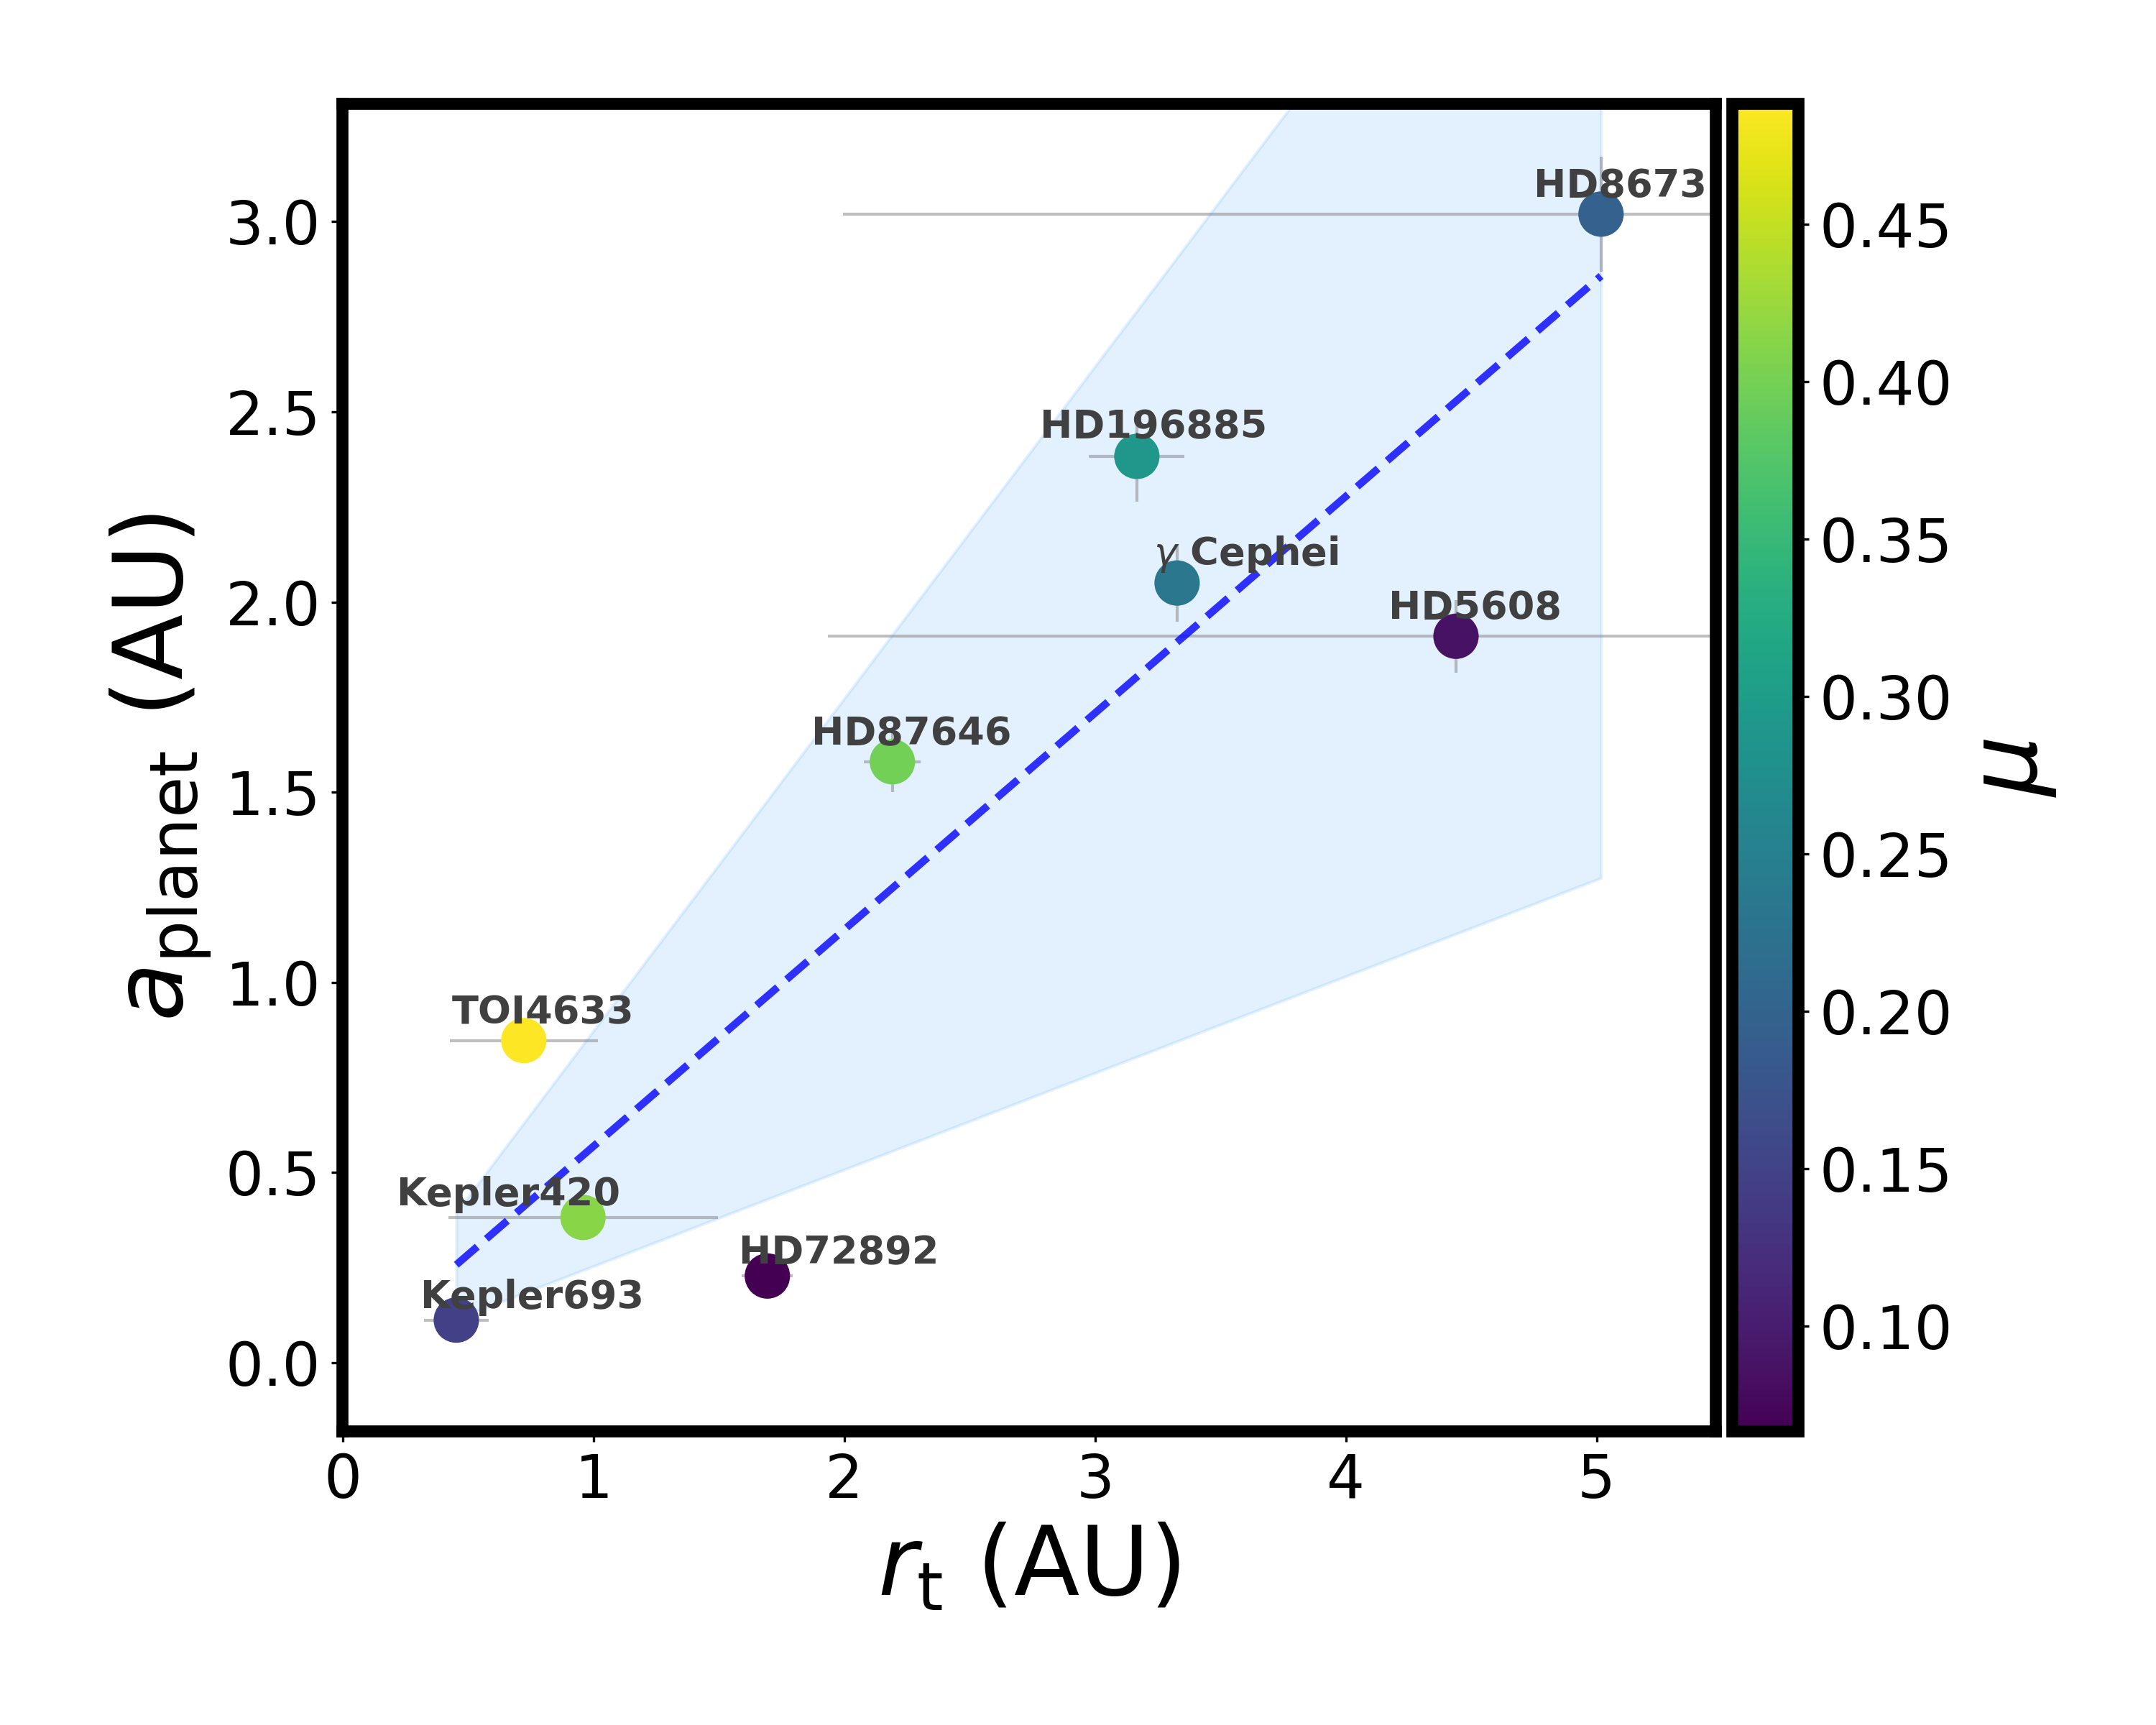
\includegraphics[width=\textwidth]{scatter_traps_group_unstable_gaints_rt_color_mu_star_all_False.png}
    \caption{Truncation radius $r_t$ versus observed planetary semi-major
    axis $a_\mathrm{planet}$ for the nine non-evolved, non-triple gas
    giants with measured eccentricity and $r_\mathrm{snow} > 0.8\,a_c$.
    \rev{The dashed line is the unweighted least-squares relation through
    the origin, $a_\mathrm{planet} = 0.569\,r_t$ ($r = 0.90$); the shaded
    band is the $\pm1\sigma$ intrinsic scatter (0.27\,dex) of the
    maximum-likelihood fit.} Colour
    encodes the companion mass ratio $\mu$. Uncertainties on the x-axis
    are propagated from observed binary parameters; uncertainties on the
    y-axis are taken as 5\% when no uncertainty in $a_\mathrm{planet}$
    was provided.}
    \label{fig:trap_vs_observed_goods}
\end{figure*}

\begin{figure}
    \centering
    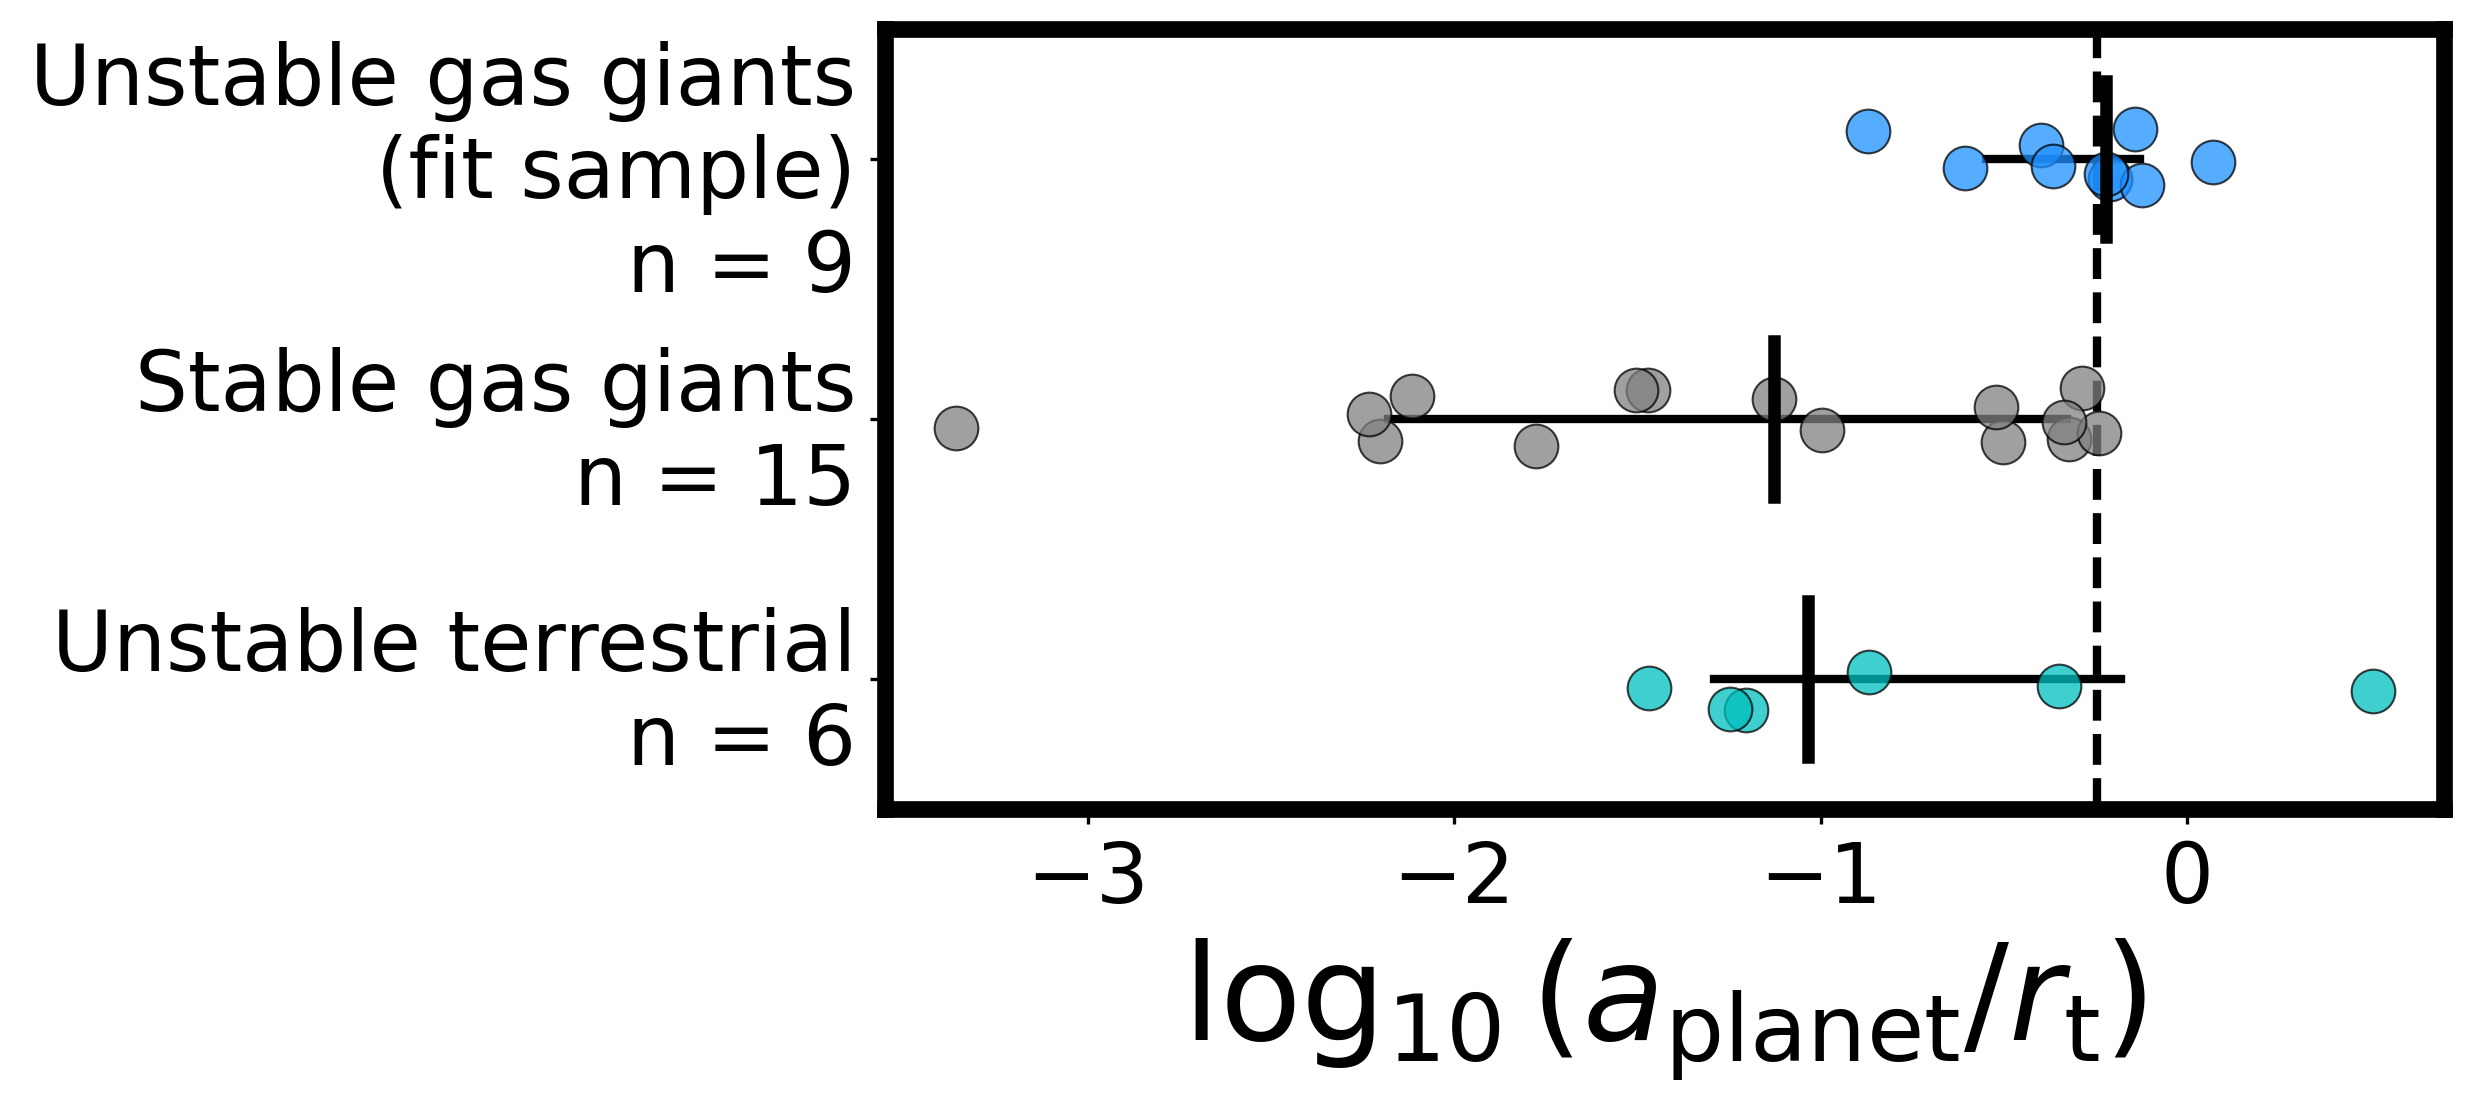
\includegraphics[width=\columnwidth]{ap_over_rt_groups.png}
    \caption{\rev{$a_\mathrm{planet}/r_t$ for the nine gas giants with
    unstable snow lines used in the fit, for gas giants with stable snow
    lines, and for terrestrial planets with unstable snow lines; only
    systems with measured $e_b$ are shown. Each point is one system
    (vertically jittered); the thick tick is the median and the bar the
    16--84\% range of each group. The dashed line marks
    $a_\mathrm{planet}/r_t = 0.569$.}}
    \label{fig:ap_over_rt}
\end{figure}

Figure~\ref{fig:trap_vs_observed_all} (Appendix~\ref{app:figs}) shows
the same relation for the full sample including evolved and triple
systems. \rev{Relative to the intrinsic scatter of the relation, the
triple system HD~28192 ($-4.0\sigma$) and $\nu$~Oct ($+2.4\sigma$) are
clear outliers, HD~59686 ($+1.5\sigma$) and $\gamma$~Leo ($-1.0\sigma$)
are marginal, and HIP~90988 and HD~145934 ($+0.8\sigma$) are consistent
with the relation. The two strongest outliers are the triple and the
host of the best-established retrograde, second-generation planet
\citep{cheng_retrograde_2025}. The exclusion of the six systems from the
fit is a priori (evolved host or companion, or a third star), not based
on their residuals, and we do not claim that evolved systems deviate as
a class.}

\rev{The relation also holds for} extreme systems like
\textit{TOI~4633}, which was suggested to be in a retrograde orbit by
\citet{Stegmann2025}. Under standard formation theory, the planet would
need to form below the snow line; \rev{its position, $1.2\,r_t$, is the
largest fraction in the sample but within the scatter of the relation.}

Using the same argument but inverting Eq.~\eqref{eq:rt}, \rev{the
relation gives the binary eccentricity for which a planet with a known
$a_\mathrm{planet}$ sits at $0.57\,r_t$, with an interval set by the
intrinsic scatter. Two systems in the sample have no measured $e_b$.
For HIP~107773 the planet would sit at $0.06\,r_t$ around a circular
binary, so the relation requires a highly eccentric one,
$e_b = 0.86$ ($0.76$--$0.92$ at one sigma, $0.60$--$0.95$ at two). The
upper end coincides with the planet's dynamical stability limit, which
lies at $e_b = 0.89$--$0.96$ depending on the criterion
\citep{Holman1999, Quarles_2020}, both extrapolated beyond $e_b = 0.8$
there; the lower end is the prediction: a measured $e_b$ below $0.6$
would contradict the relation. The caveat is that
HIP~107773 is a K giant, i.e. one of the evolved hosts excluded from the
calibration. For TOI~1736 the planet already sits at $0.59\,r_t$ around
a circular binary, and the inversion gives only $e_b \lesssim 0.4$,
which the planet's stability requires anyway, so the relation adds
nothing there.}

\subsection{No pressure maximum at the truncation edge}
\label{sec:model_results}

\rev{Figure~\ref{fig:model} shows the disc model of Sect.~\ref{sec:model}
for $\gamma$~Cephei. In every run the pressure decreases monotonically
with radius: its logarithmic slope is $-2.75$ inside the disc and
steepens to below $-4$ beyond $\approx1.05\,r_t$. Removing gas at the
edge, or adding it at $r_t$ or at $0.5\,r_t$, changes the slope but never
its sign, for a reason that does not depend on the model. In a thin,
viscously steady disc the angular-momentum balance reads
\citep{Lynden-Bell1974, Kanagawa2015_torque_exp}
\begin{equation}
\frac{\mathrm{d}\Gamma}{\mathrm{d}r} = \dot{M}\,\frac{\mathrm{d}\ell}{\mathrm{d}r}
+ 2\pi r\,\Sigma\,\Lambda, \qquad \Gamma = 3\pi\nu\Sigma r^2\Omega_K,
\label{eq:am_balance}
\end{equation}
where $\Gamma$ is the viscous angular-momentum flux, $\dot{M}$ the inward mass
flux, $\ell = r^2\Omega_K$ and $\Lambda$ the tidal torque per unit mass.
With $\nu = \alpha c_s^2/\Omega_K$ \citep{Shakura1973}, $T \propto
r^{-\beta}$ and $P \propto \Sigma c_s\Omega_K$, the pressure slope is
\begin{equation}
\frac{\mathrm{d}\ln P}{\mathrm{d}\ln r} =
\frac{\mathrm{d}\ln \Gamma}{\mathrm{d}\ln r} + \frac{\beta}{2} - \frac{7}{2},
\label{eq:pressure_slope}
\end{equation}
so a maximum requires $\Gamma$ to rise outward at least as $r^{3}$ for
$\beta \le 1$ \citep{Chiang1997}. Accretion alone gives
$\mathrm{d}\ln \Gamma/\mathrm{d}\ln r \to 1/2$, hence the slope of $-11/4$
for $\beta = 1/2$. The companion's torque is negative everywhere inside
its orbit, since the gas there orbits faster than the companion and is
dragged back by it, so the torque term of Eq.~\eqref{eq:am_balance},
$2\pi r\Sigma\Lambda$, is negative and only lowers
$\mathrm{d}\Gamma/\mathrm{d}r$, steepening the pressure decline: this is
the truncation edge. A positive $\Lambda$, which the companion exerts only
outside its own orbit, is needed for a maximum, and that is where the
single maximum in the simulations of \citet{Marzari2025, Marzari2025b}
sits, at the inner rim of the circumbinary disc. Inflow adds mass, not
angular momentum, and does not change this. The isolated disc drains in $\sim10^5$\,yr, and the inflow-fed
disc settles within $10^5$\,yr to $1\times10^{-3}\,M_\odot$
($\alpha = 10^{-2}$) or $8\times10^{-3}\,M_\odot$ ($\alpha = 10^{-3}$),
in line with \citet{Marzari2025}. The dust follows the gas: the
dust-to-gas ratio is flat at $\approx0.004$ for $\alpha = 10^{-2}$
(Stokes numbers of $10^{-3}$) and $\approx10^{-4}$ for
$\alpha = 10^{-3}$ (Stokes numbers of $10^{-2}$), with at most a
factor-of-two enhancement between 0.6 and $0.95\,r_t$ where freshly
delivered grains still drift slowly. Half of the delivered dust is
stripped at the edge; the other half, $\approx30\,M_\oplus$\,Myr$^{-1}$,
drifts through every radius inside $r_t$ to the star. Since the
dust-to-gas ratio never approaches unity, feedback of the dust on the
gas cannot create a maximum either. The other eight fit systems, run
with inflow at $r_t$ and $\alpha = 10^{-2}$, behave identically despite
spanning $\mu = 0.07$--$0.49$ and $e_b = 0.31$--$0.91$: none has a
pressure maximum, the inner slope is $-2.75$ in all of them, the
dust-to-gas ratio is flat at 0.004--0.005 with its maximum at the inner
boundary, and the pebble flux is $35\,M_\oplus$\,Myr$^{-1}$ in each,
because the delivery rate, not the binary, sets it. The ballistic
calculation gives the same picture for all nine fit systems:
inflowing material enters the
host's disc with a broad range of angular momenta, circularising between
0.05 and $1.4\,r_t$ (16th to 84th percentiles; medians of
0.5--0.7\,$r_t$), with no preferred radius and no dependence on where the
planet is observed. Delivered solids therefore drift through the edge
rather than collecting at it, and the candidate of
Sect.~\ref{sec:mechanism} is ruled out for an axisymmetric disc with
uniform viscosity. Processes outside that framework remain untested by
this model: heating of the edge by companion-driven spiral shocks, which
could invert the temperature gradient over the last scale heights, and
the non-local deposition of the tidal torque by the same waves, both of
which require a radiative two-dimensional model, and non-axisymmetric
concentration in an eccentric disc, which the three-dimensional models of
\citet{Marzari2025b} make weak ($e_\mathrm{disc} \lesssim 0.03$).}

\begin{figure*}
    \centering
    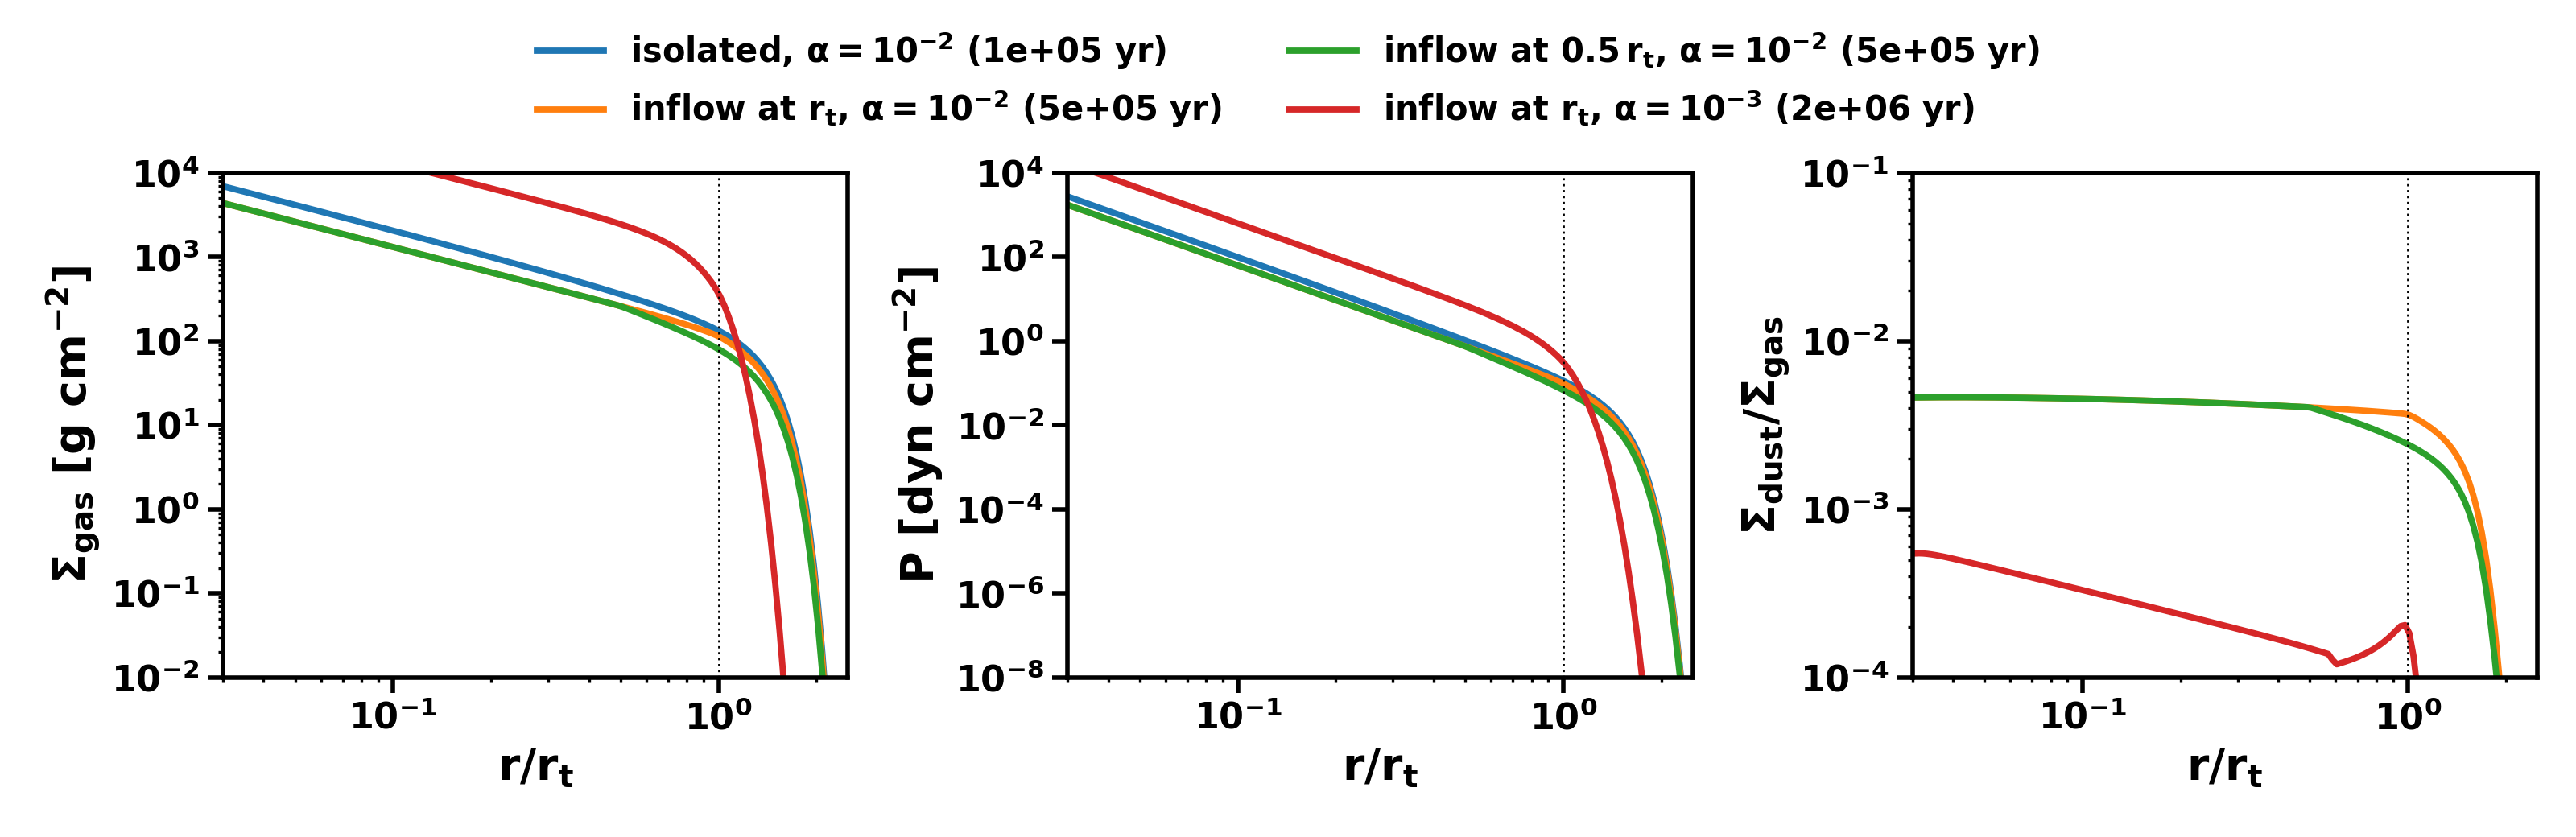
\includegraphics[width=\textwidth]{model_gcep.png}
    \caption{\rev{One-dimensional model of the circumprimary disc of
    $\gamma$~Cephei (Sect.~\ref{sec:model}): gas surface density (left),
    midplane pressure (middle) and dust-to-gas ratio (right) against
    radius in units of the truncation radius of Eq.~\eqref{eq:rt} (dotted
    line), for an isolated disc and for discs fed at
    $2\times10^{-8}\,M_\odot$\,yr$^{-1}$ at $r_t$ or at $0.5\,r_t$, with
    $\alpha = 10^{-2}$ or $10^{-3}$. The isolated disc is shown at
    $10^5$\,yr, the others in steady state. The pressure has no local
    maximum in any case.}}
    \label{fig:model}
\end{figure*}

%% =========================================================================
\section{Discussion}
\label{sec:discussion}
%% =========================================================================

We have shown that gas-giant planets exist in binary systems where
standard formation theory predicts they cannot form, and that their
positions are well described by a linear relation with the tidal
truncation radius. \rev{This provides an empirical constraint on where
gas giants form in binary systems, with a scatter of a factor of two
about the relation.}

Planet-formation theory and modelled processes are notoriously difficult
to verify observationally, given the short timescales involved and the
challenges of probing the early stages of disc evolution at high
resolution. The study of snow-line-unstable gas-giant systems in
binaries provides a unique empirical probe into these processes, allowing
quantitative tests of planet formation theory \rev{at the population
level}.

We caution that the current sample is small (nine systems used for
calibration) \rev{and that the relation has an intrinsic scatter of a
factor of two. The model of Sect.~\ref{sec:model_results} rules out one
candidate explanation: tidal truncation does not create a pressure
maximum, in our one-dimensional discs or in the published two- and
three-dimensional ones \citep{Muller2012, Jordan2021, Marzari2025,
Marzari2025b}, and the solids delivered by circumbinary inflow do not
collect anywhere in particular. What the correlation then constrains is
the formation process itself. The global models of \citet{Venturini2026}
and \citet{Ronco2026} contain the ingredients our model lacks, namely
pebble accretion onto a growing core and its migration in an
inflow-fed, truncated disc; because the disc mass, the pebble flux and
the migration rate in such a disc all scale with its size, their final
planet positions should scale with $r_t$, and the coefficient of
$\approx0.6$ and its scatter are a direct test of them. Near a disc
edge the migration torque reverses, because the outer Lindblad
resonances of a planet fall in the depleted region, the counterpart of
the inner-edge traps of \citet{Masset2006}. Where this leaves a
gap-opening giant in a truncated, inflow-fed disc has not been
computed, and is the natural first test of the scaling. In our model
the pebble flux through the disc is $\approx30\,M_\oplus$\,Myr$^{-1}$ at
the measured inflow rate, with Stokes numbers of $10^{-3}$--$10^{-2}$,
which places core growth in the slow, three-dimensional pebble-accretion
regime; whether a core reaches the runaway mass within the disc lifetime
is the question those models answer and ours does not.}
Observational evidence from spatially resolved circumstellar discs in
binary systems -- such as HD~100453 \citep[cf.][]{Cuello2025} -- would
also provide valuable constraints.

\rev{Our truncation radii assume coplanar discs. Misaligned
circumstellar discs are tidally warped and precess \citep{Larwood1996,
Fragner2010}, can be disrupted near their outer edge \citep{Dogan2015},
and are truncated further out, because the resonant torques weaken with
inclination, by about 20\% at $90^\circ$ for an equal-mass binary
\citep{Miranda2015, Lubow2015}. Only four of our 17 systems have a
catalogued mutual inclination, and the prescription of
\citet{Manara2019A&A...628A..95M} evaluated as in
Appendix~\ref{app:manara} does not carry an inclination term. For the
inclinations in our sample the coplanar $r_t$ would therefore be an
underestimate by at most tens of percent, well inside the intrinsic
scatter of the relation.}

%% =========================================================================
\section{Conclusions}
\label{sec:conclusions}
%% =========================================================================

\rev{The sample of gas giants with unstable snow lines is difficult to
explain by core accretion beyond the water snow line under their binary
architectures, and calls for alternative formation or evolutionary
pathways. Their positions correlate with the tidal
truncation radius set by the stellar companion
($a_\mathrm{planet} = 0.57\,r_t$, $r = 0.90$, intrinsic scatter
0.27\,dex), while gas giants with stable snow lines show no such
relation; the triple system HD~28192 and the retrograde-planet host
$\nu$~Oct are the clearest outliers. A one-dimensional gas--dust model
of the truncated disc, with and without circumbinary inflow, produces no
pressure maximum at the edge and no accumulation of delivered solids, so
a dust trap at the truncation edge of an axisymmetric disc with uniform
viscosity is not the explanation. The planets sit
at a fixed fraction of the disc size set by the companion, and that
scaling is the constraint that formation models for planets in close
binaries must reproduce. Inverted, the relation predicts a highly
eccentric companion orbit for HIP~107773 ($e_b = 0.76$--$0.92$), which
a measurement of that orbit would test.}

\begin{acknowledgements}
\rev{IK is supported by the Azrieli Graduate Fellowship. This work used the catalogue of planets in binary systems of
\citet{Thebault2025}, the MIST stellar evolution grid
\citep{Choi2016} accessed through \texttt{kiauhoku}, the DustPy disc
code \citep{Stammler2022}, and the \texttt{numpy}, \texttt{scipy},
\texttt{pandas}, \texttt{astropy}, \texttt{numba} and
\texttt{matplotlib} packages. The analysis and disc-model code, the
processed catalogue and the model outputs underlying this article are
available from the corresponding author on request.}
\end{acknowledgements}

%% -------------------------------------------------------------------------
\bibliographystyle{plainnat}   %% aa.bst not required; plainnat gives same author-year format
\bibliography{main}
%% -------------------------------------------------------------------------

%% =========================================================================
%% APPENDICES -- must come after \bibliography in aa.cls
%% =========================================================================
\begin{appendix}

\section{Supplementary figures}
\label{app:figs}

\begin{figure}
    \centering
    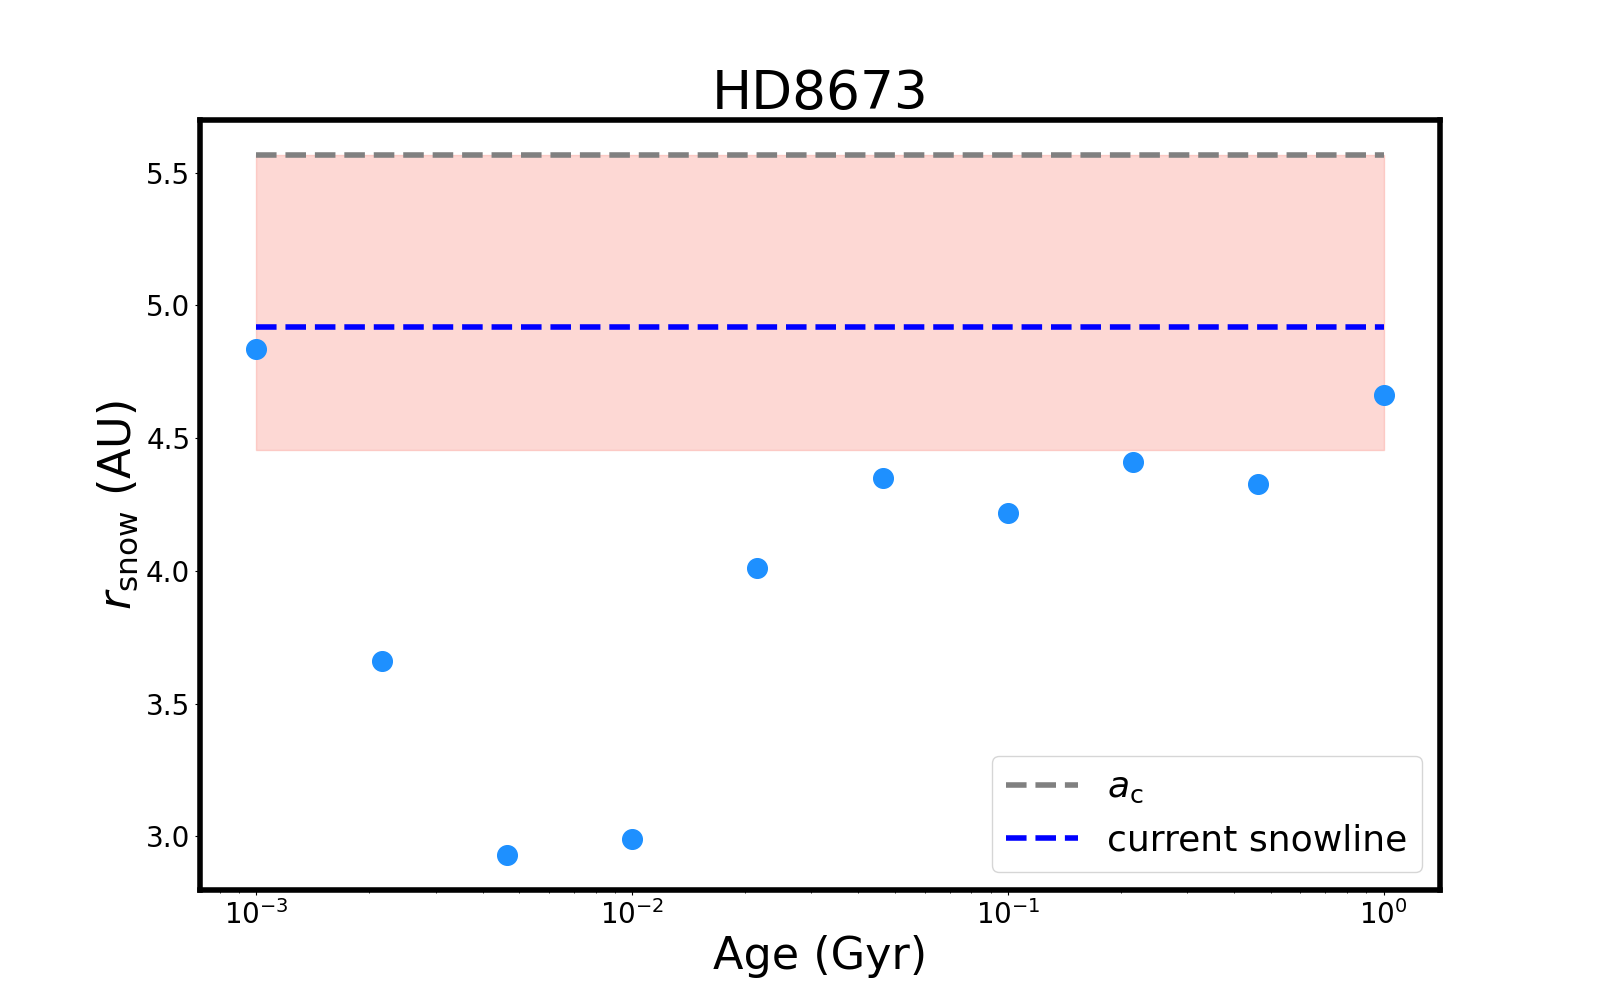
\includegraphics[width=\columnwidth]{snowline_evolution.png}
    \caption{Example of snow-line evolution for \textit{HD~8673}. The
    position of the snow line at different ages was calculated \rev{from
    MIST stellar tracks \citep[built with MESA;][]{Choi2016, Paxton2011,
    Jermyn2023}}. The shaded pink region marks the
    unstable zone ($r_\mathrm{snow} > 0.8\,a_c$).}
    \label{fig:snowline_evolution}
\end{figure}

\begin{figure}
    \centering
    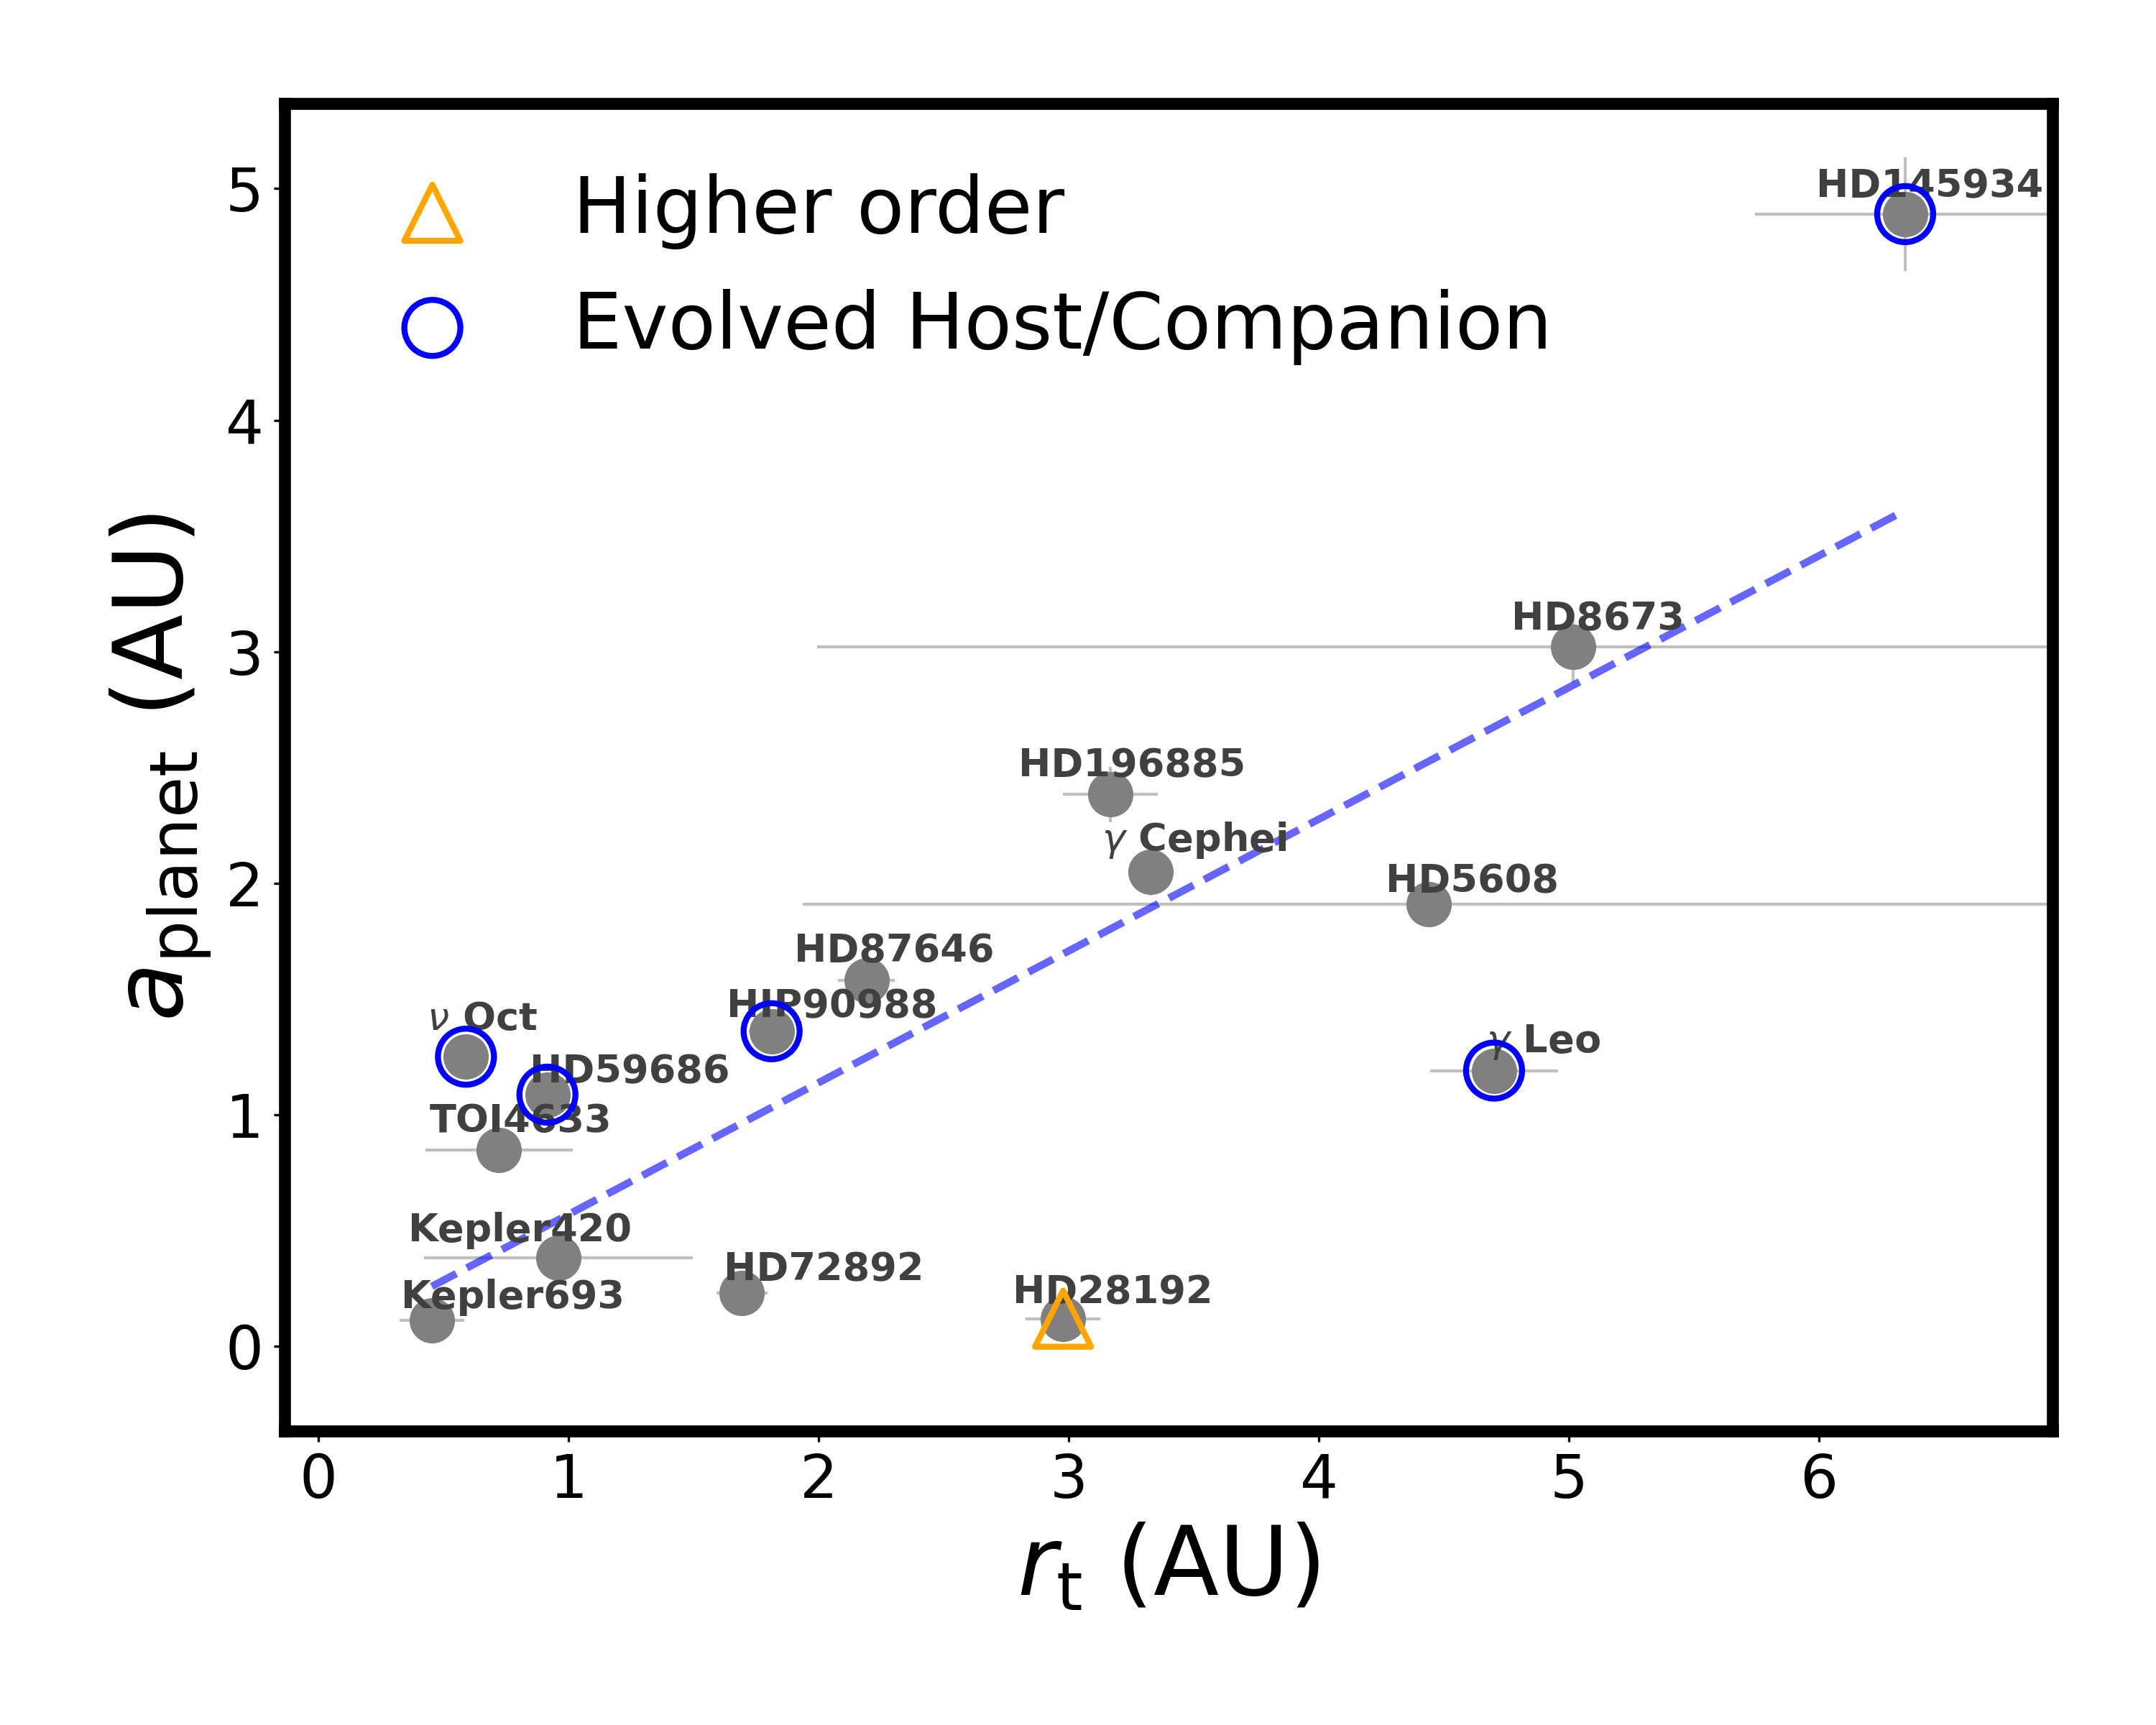
\includegraphics[width=\columnwidth]{scatter_traps_group_unstable_gaints_rt_color_None_all_True.png}
    \caption{Same as Fig.~\ref{fig:trap_vs_observed_goods} but for the
    full sample. Triple systems are marked with triangles; evolved
    systems with circles.}
    \label{fig:trap_vs_observed_all}
\end{figure}

\begin{figure}
    \centering
    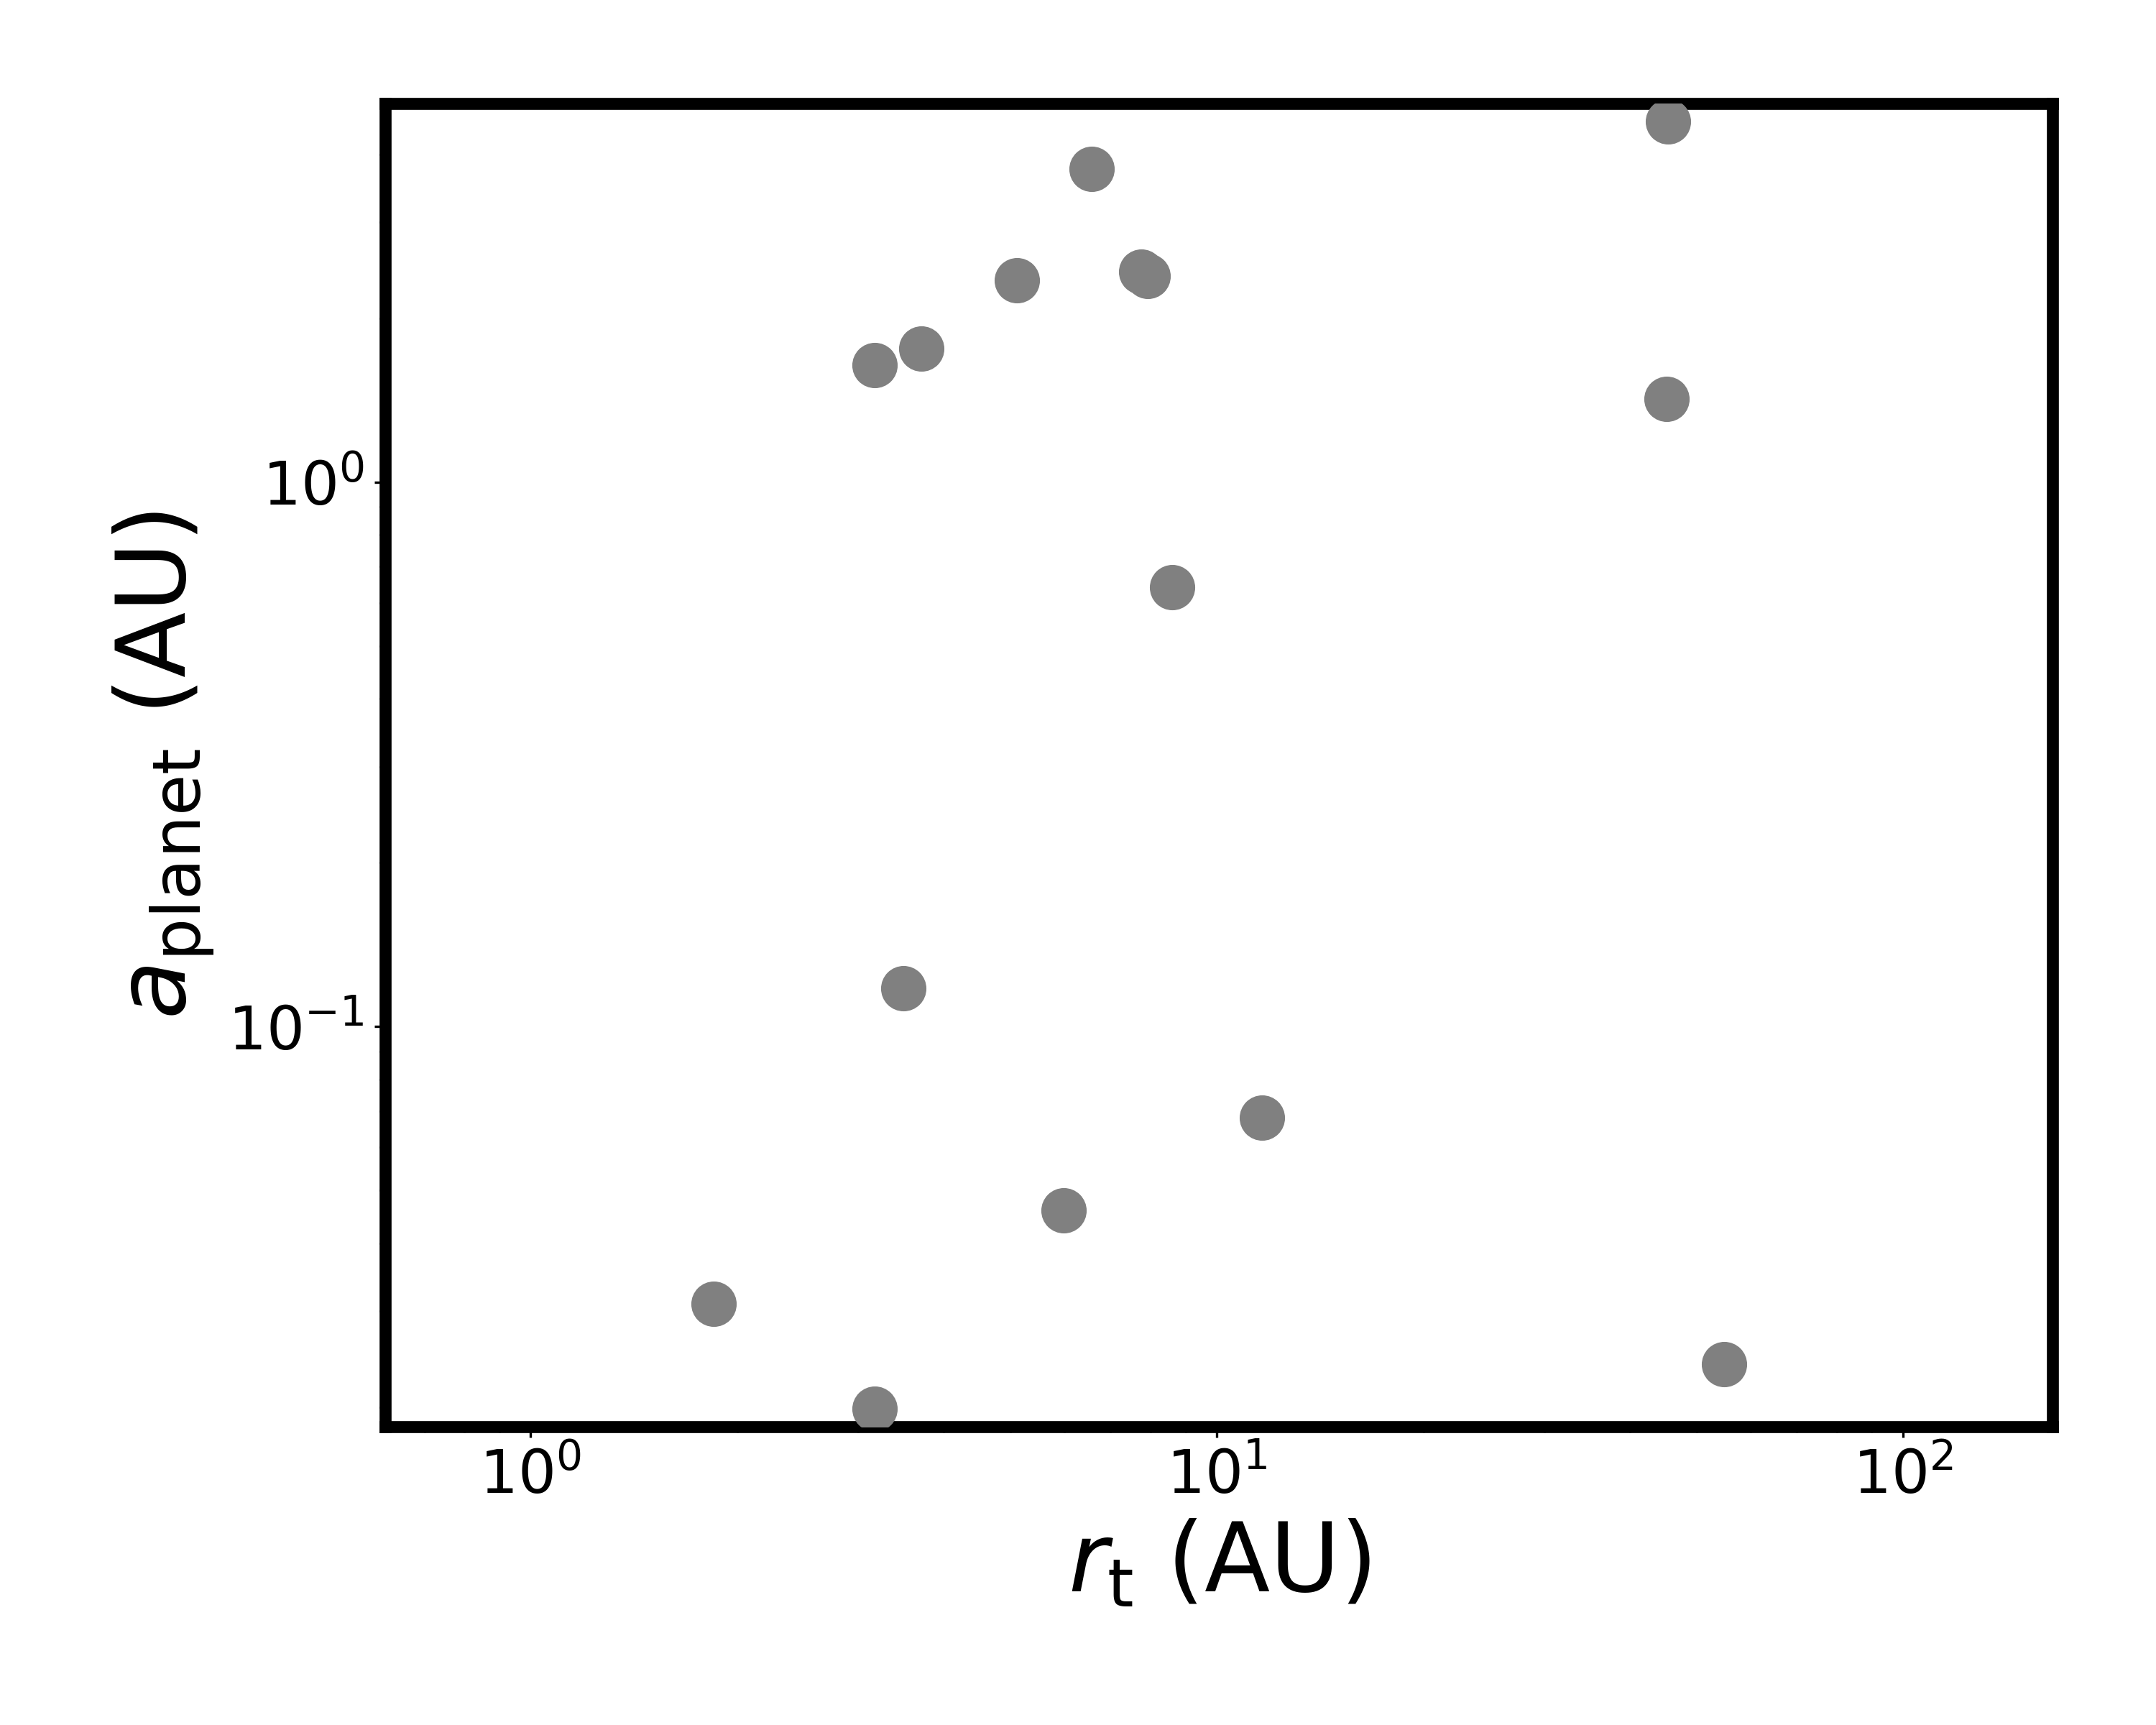
\includegraphics[width=\columnwidth]{scatter_traps_group_stable_gaints_rt_color_None_all_True.png}
    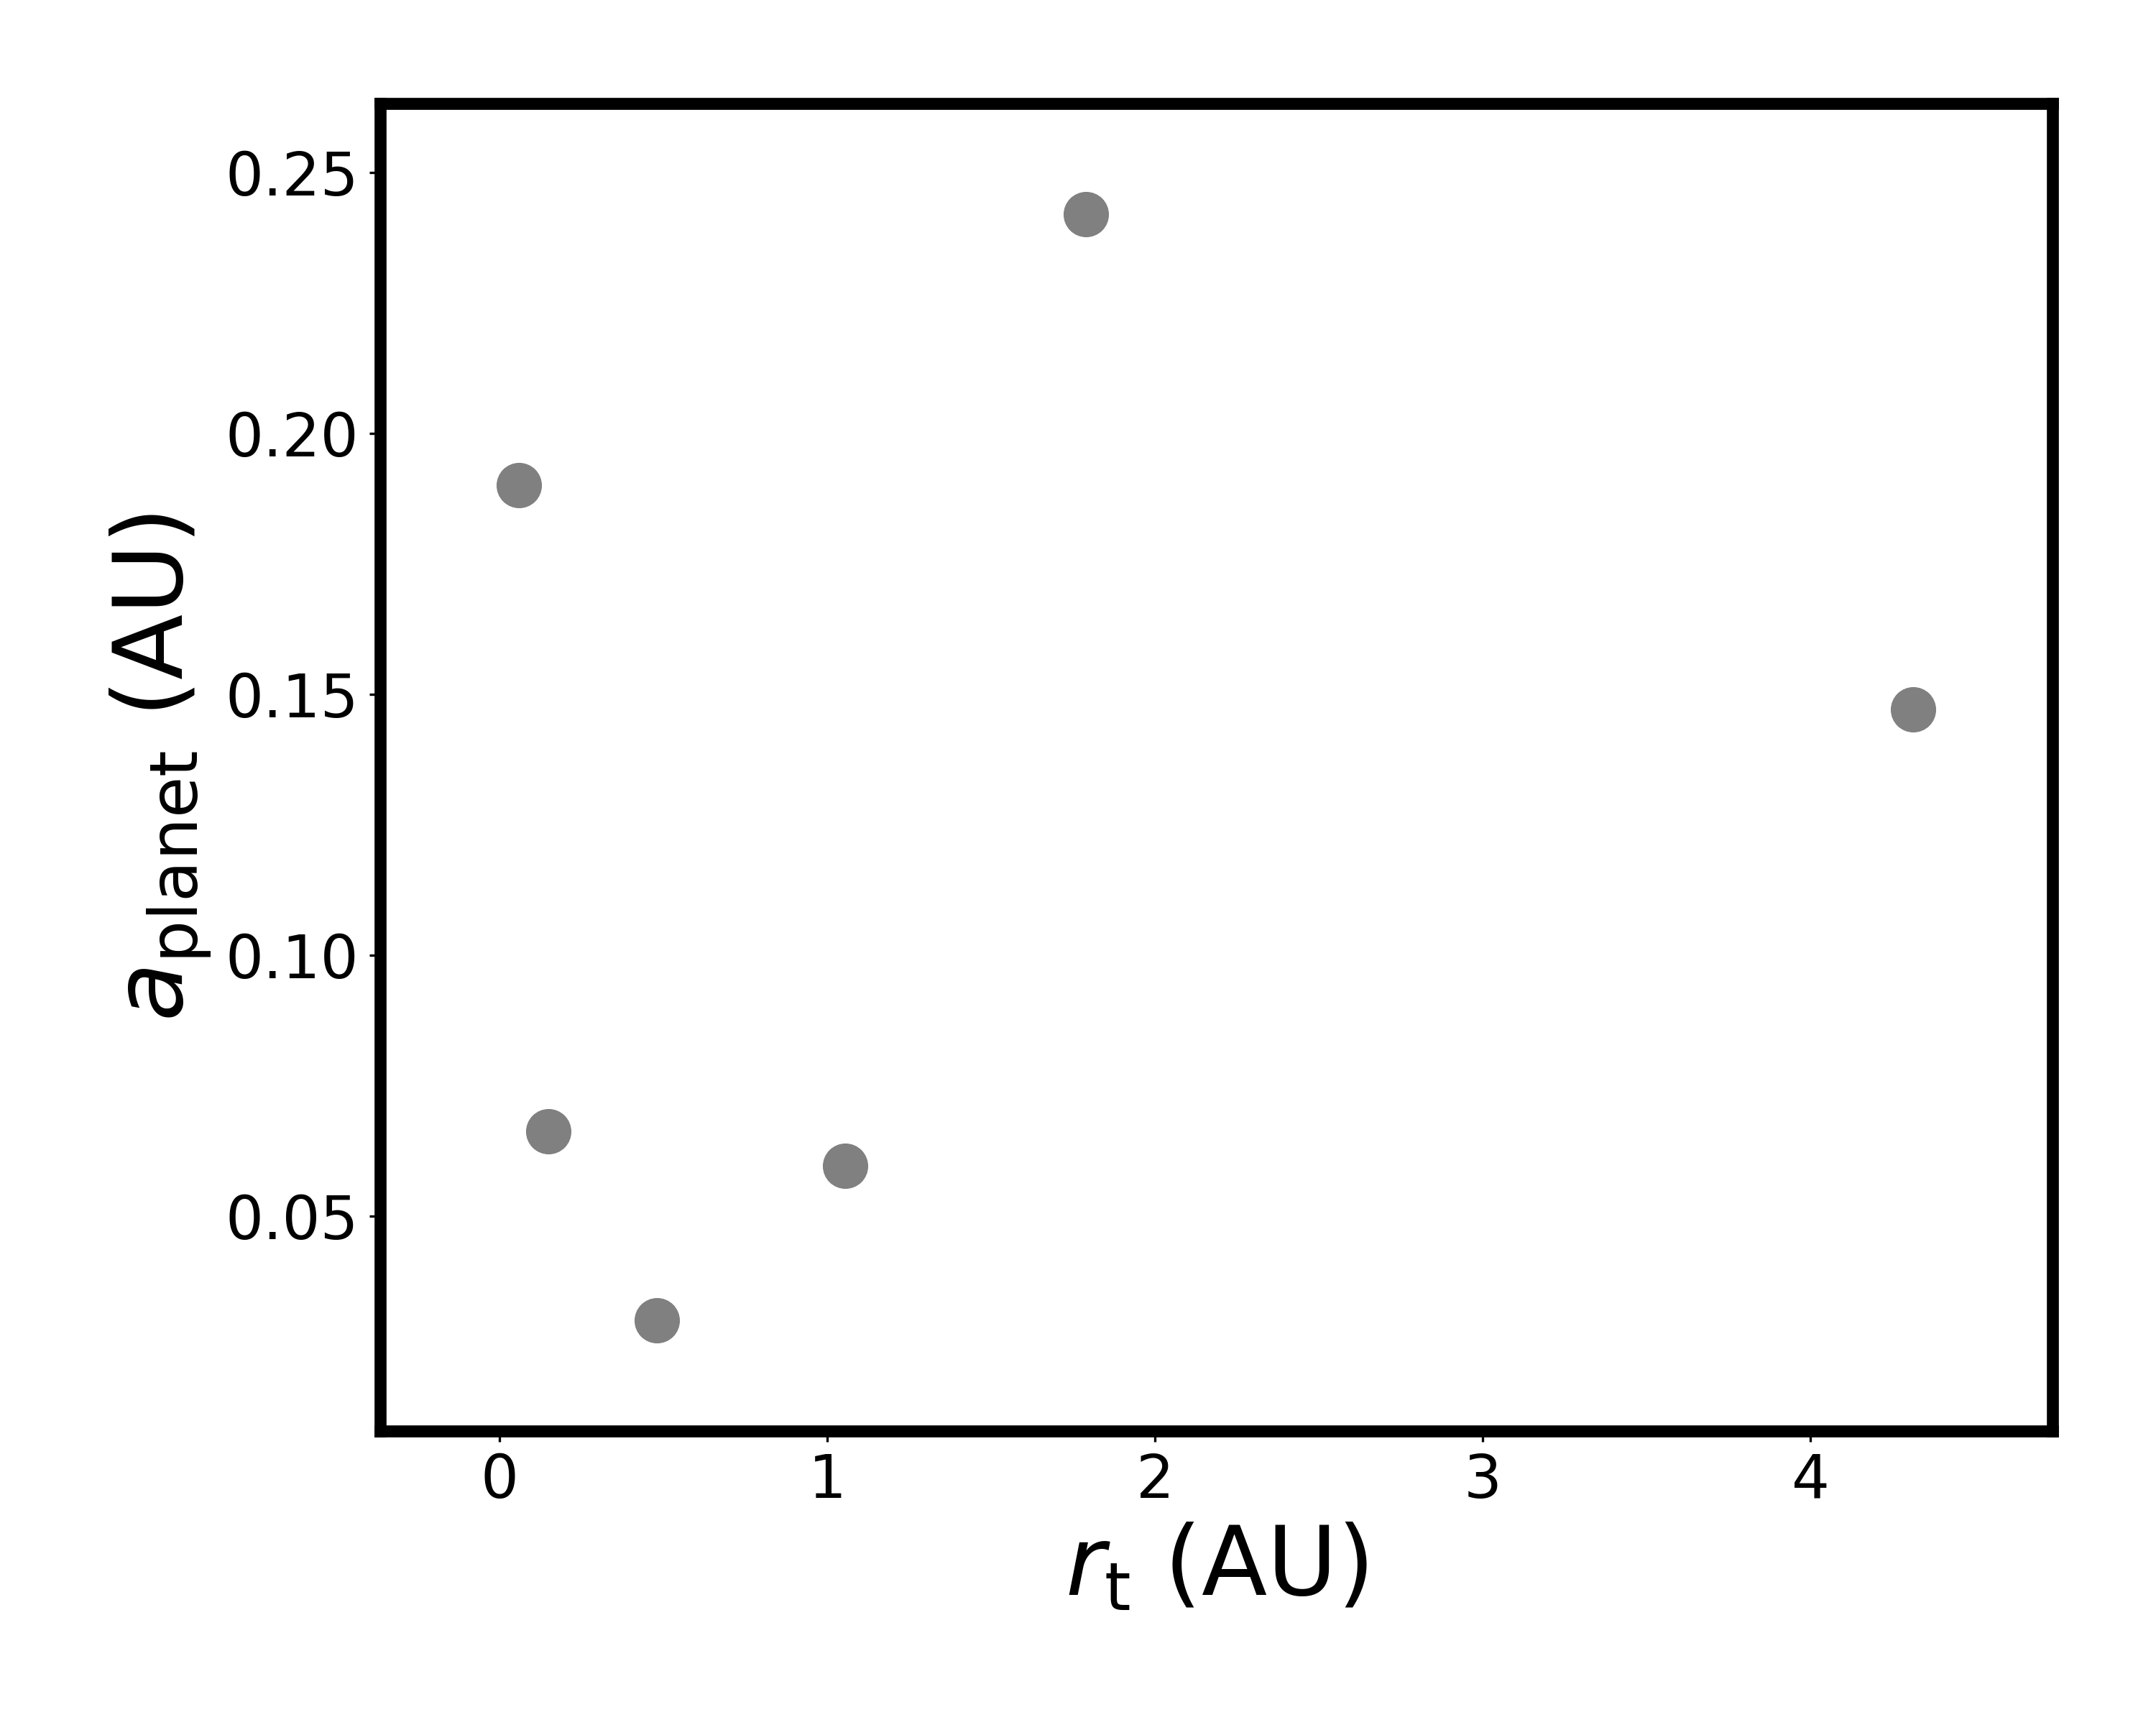
\includegraphics[width=\columnwidth]{scatter_traps_group_unstable_terrestrial_rt_color_None_all_True.png}
    \caption{$r_t$ vs $a_\mathrm{planet}$ for gas giants with stable
    snow lines (upper panel) and terrestrial planets with unstable snow
    lines (lower panel). Only systems with measured eccentricity are
    shown.}
    \label{fig:trap_vs_observed_stable_giants_unstable_terrestrial}
\end{figure}

\begin{figure*}
    \centering
    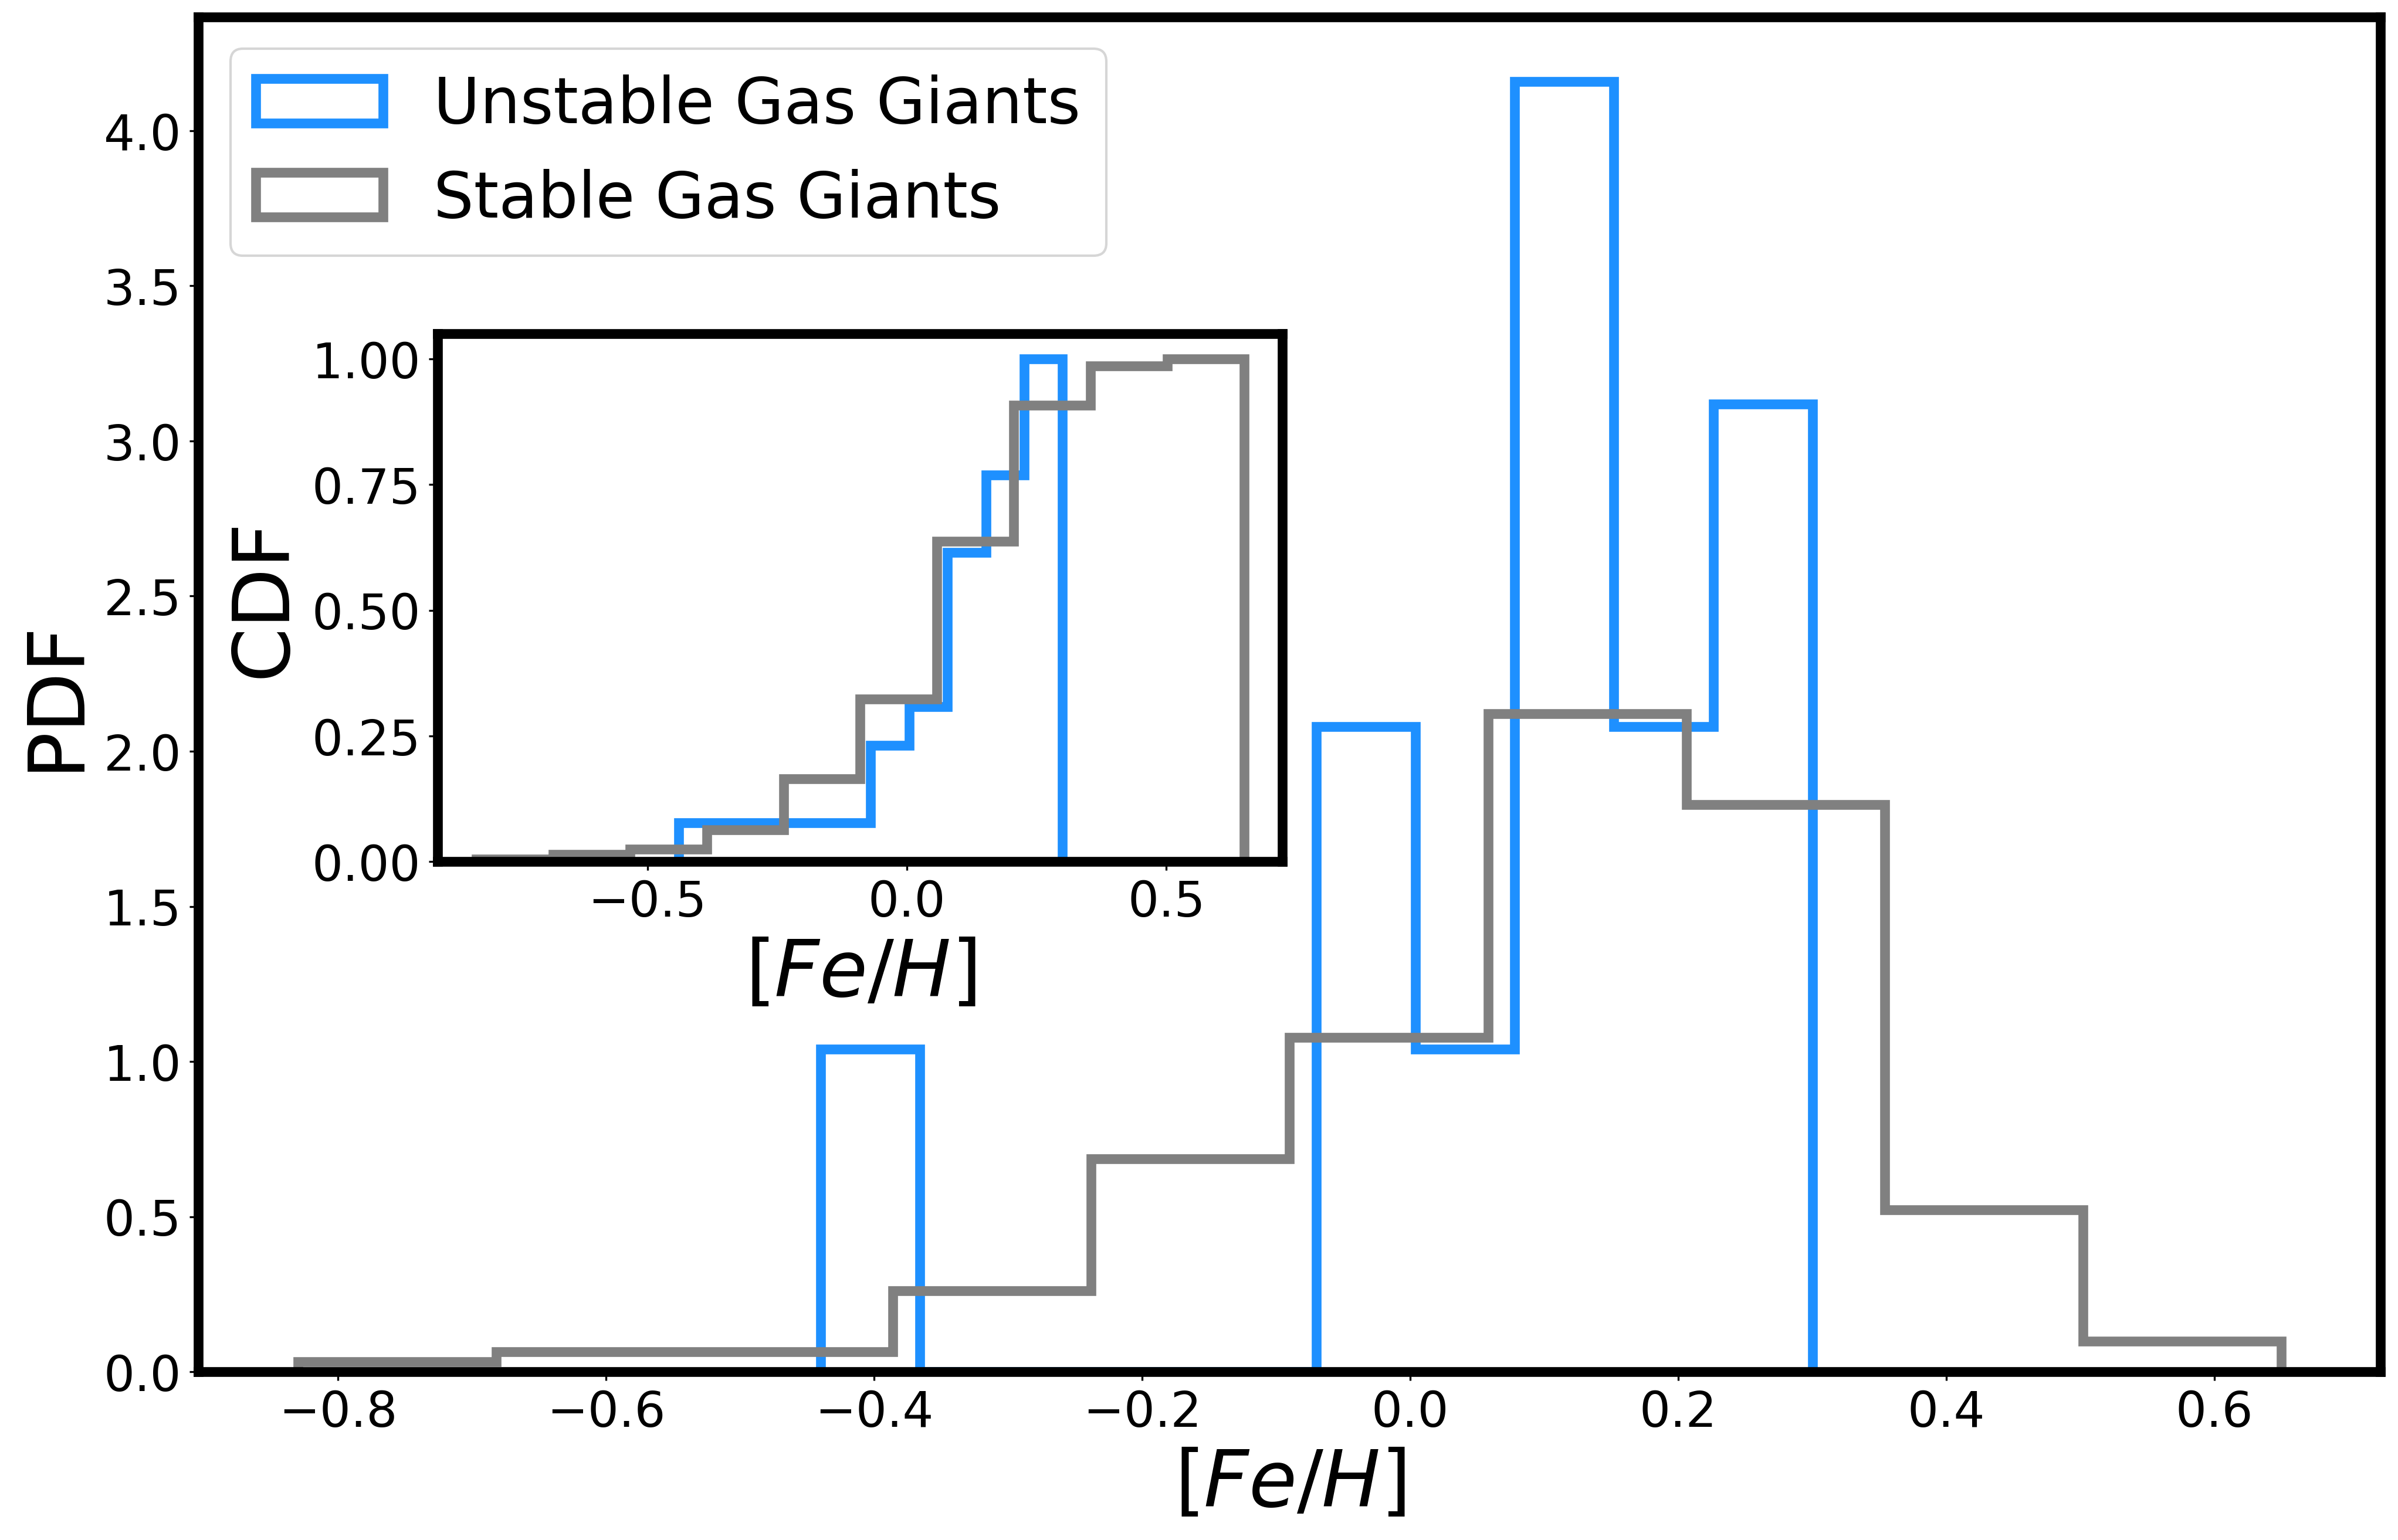
\includegraphics[width=0.48\textwidth]{gas_giant_unstable_vs_gas_giant_stable_x_best_metallicity_value.png}
    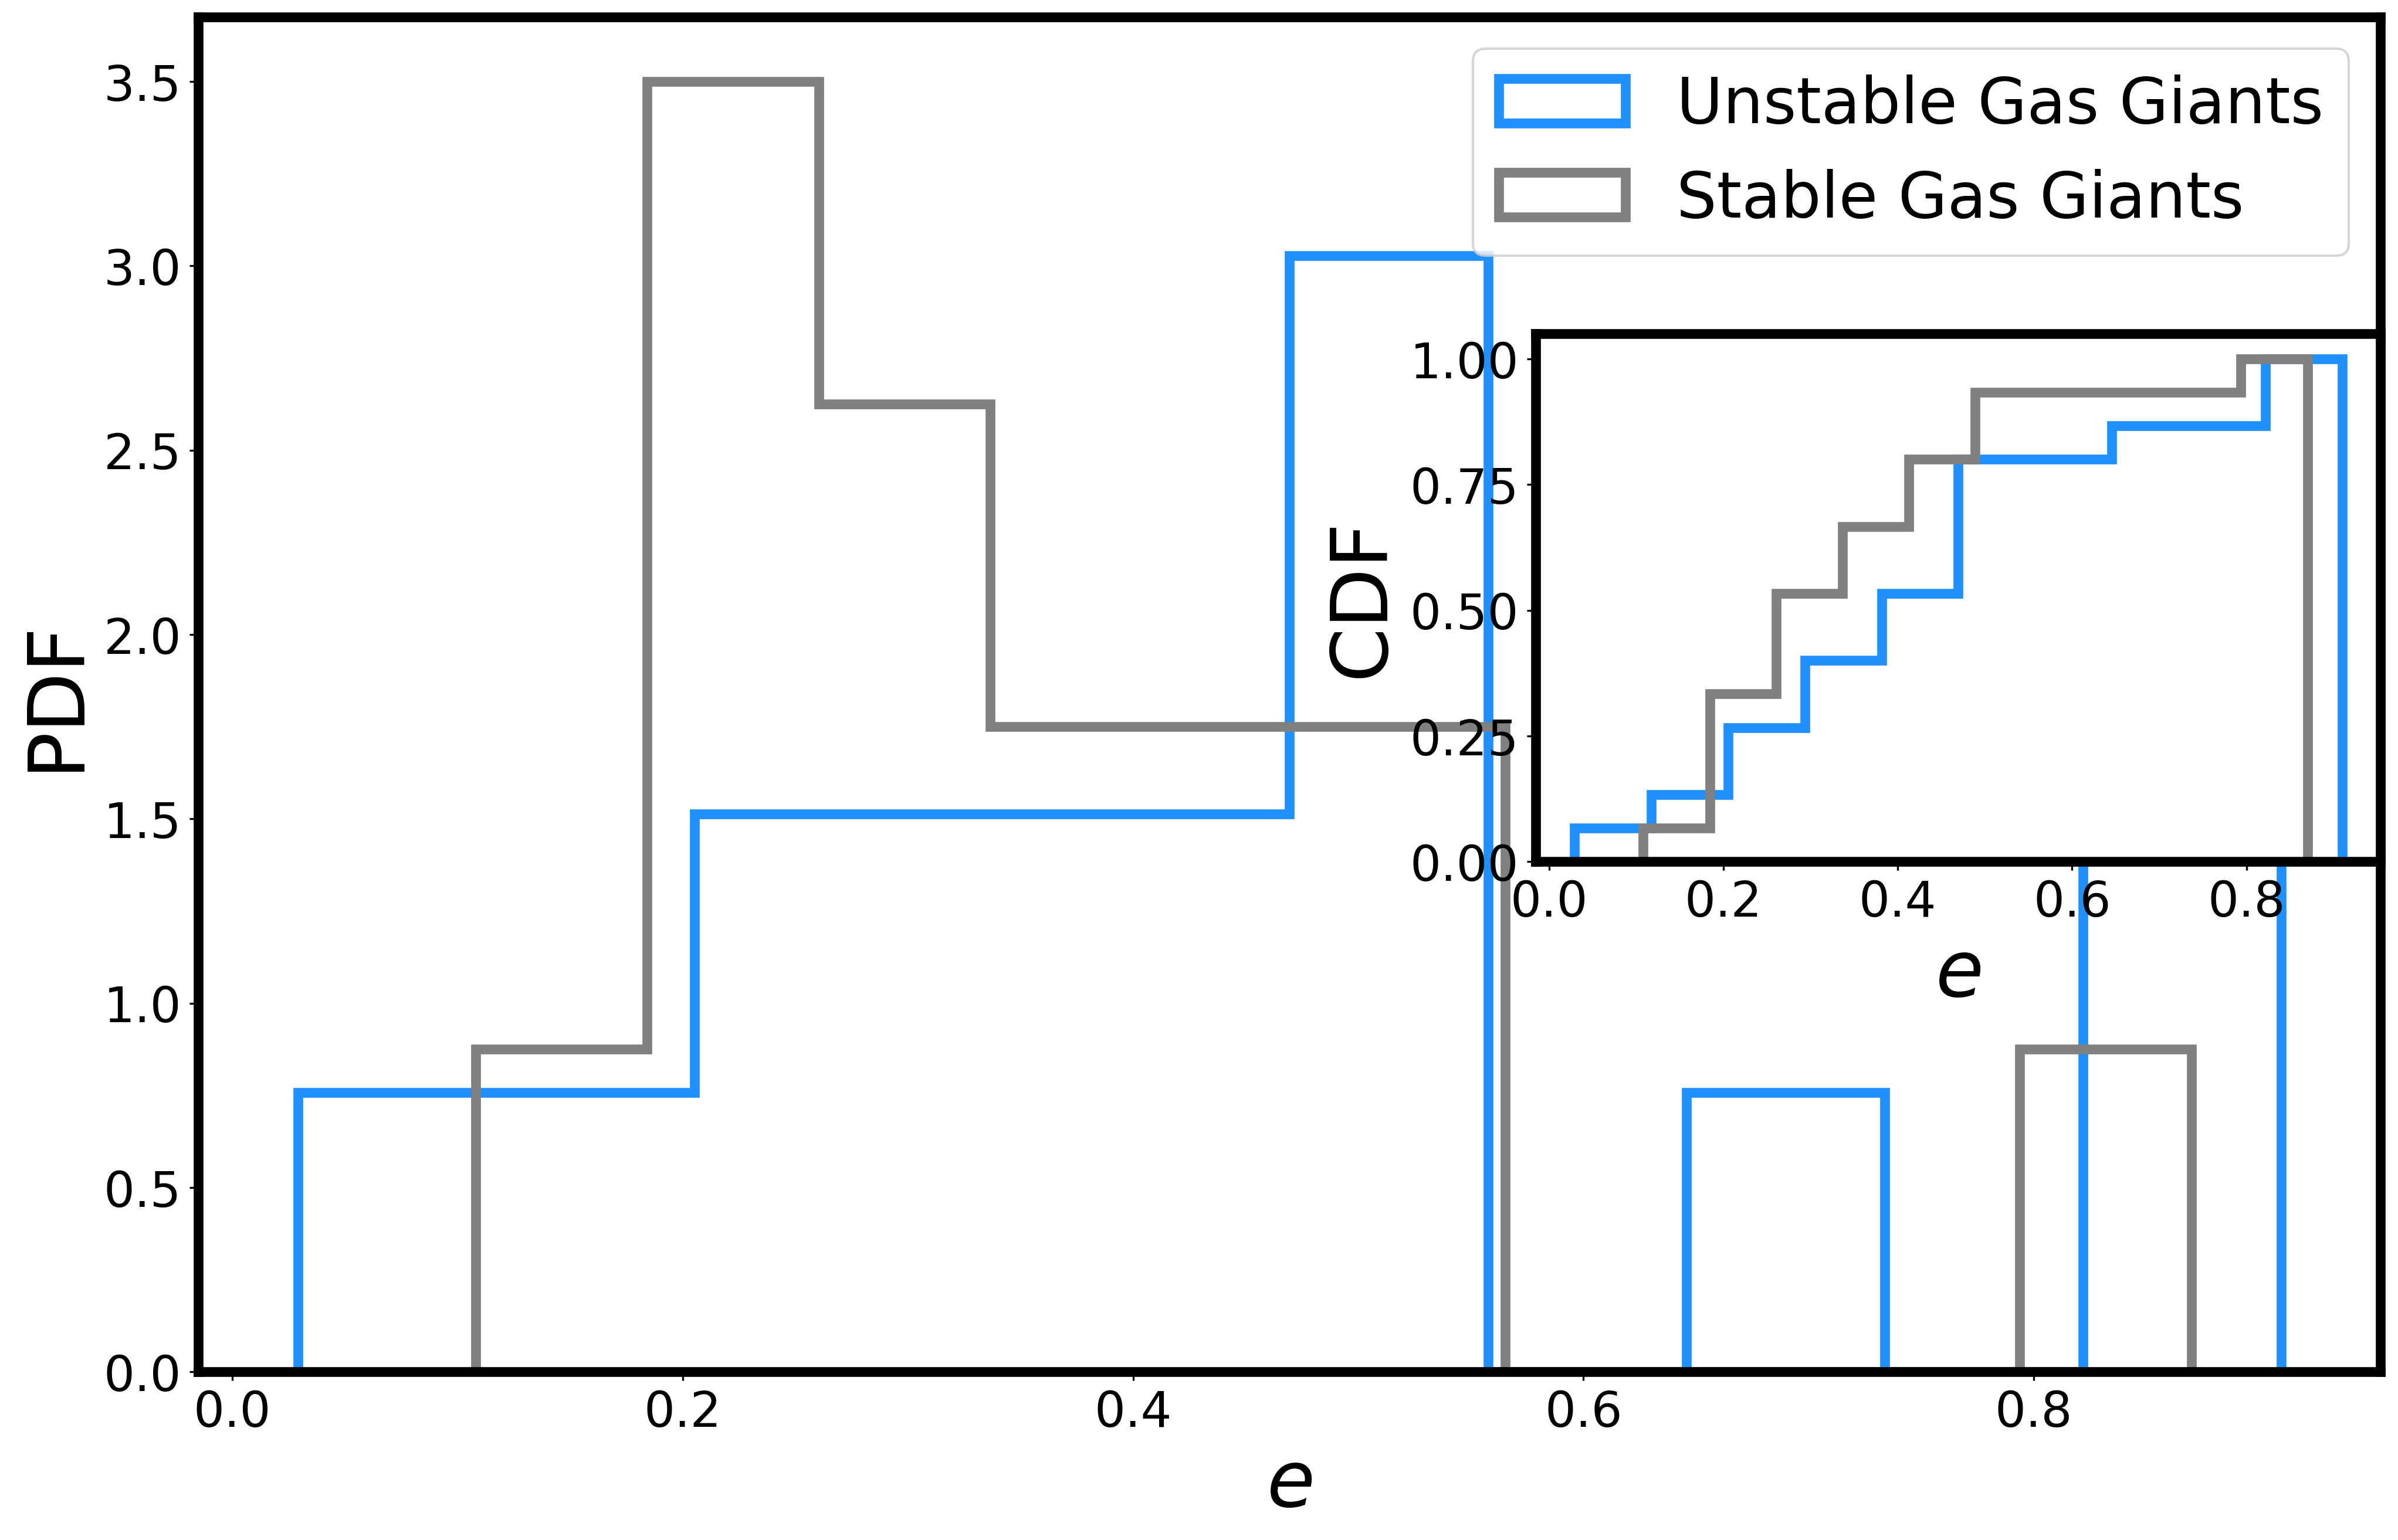
\includegraphics[width=0.48\textwidth]{gas_giant_unstable_vs_gas_giant_stable_x_eccentricity.png}
    \caption{Comparison of metallicity (left) and eccentricity (right)
    distributions between gas giants with unstable (blue) and stable
    (grey) snow lines. Insets show the cumulative distribution function.
    Kolmogorov--Smirnov p-values: \rev{0.64 (metallicity), 0.68
    (eccentricity)}, consistent with the two samples being drawn from the
    same parent distribution.}
    \label{fig:feh_e_hists}
\end{figure*}

%% -------------------------------------------------------------------------
\section{Sensitivity to truncation-radius prescription}
\label{app:manara}

As mentioned in Sect.~\ref{sec:mechanism}, we used Eq.~\eqref{eq:rt}
for the truncation radius due to its simplicity and independence from
the viscosity parameter. To assess sensitivity to this choice, we
repeated the analysis using the observationally calibrated expression of
\citet{Manara2019A&A...628A..95M}\rev{, their Eq.~C.3:}
\begin{equation}\label{eq:rt_manara}
    \frac{r_{t}}{a_b} = R_{\rm RL}\!\left(b\cdot e_b^c + 0.88\,
    \revm{\mu^{0.01}}\right),
\end{equation}
where $b$ and $c$ are parameters fitted to \citet{Artymowicz1994}
results\rev{, interpolated in $\mu$ and in the disc Reynolds number from
their Table~C.1. Here $a_b$ is the true binary semi-major axis listed in
the catalogue, so the orbital-phase factor of their Eq.~8, which converts
to a projected separation and reduces to $1/(1 \pm e_b)$ at the orbital
extremes, is not applied; the inclination enters only through that
factor, so Eq.~\eqref{eq:rt_manara} carries no inclination dependence.
For our fit sample Eq.~\eqref{eq:rt_manara} gives $r_t$ larger than
Eq.~\eqref{eq:rt} by a median factor of 1.5, essentially because the
$(1-e_b)^{1.2}$ dependence of Eq.~\eqref{eq:rt} is steeper than the
$b\,e_b^c$ term. The correlation is unchanged (Spearman $\rho = 0.87$ by
construction of the near-proportional radii) and the fit through the
origin gives $a_\mathrm{planet} = (0.375 \pm 0.039)\,r_t$ with the same
intrinsic scatter (0.24\,dex). The existence of the relation therefore
does not depend on the truncation prescription, but the coefficient
does, and the value of 0.57 should be understood as specific to the
\citet{Pichardo2005} radius. The same holds for the simplest
alternative: the binary pericentre distance $a_b(1-e_b)$ alone
correlates with the planet positions at least as well as
Eq.~\eqref{eq:rt} ($r = 0.95$ against $0.90$; rms scatter about
proportionality 0.22 against 0.28\,dex), with
$a_\mathrm{planet} \approx 0.17\,a_b(1-e_b)$, so the Roche-lobe and
$(1-e_b)^{0.2}$ factors of Eq.~\eqref{eq:rt} are not resolved by nine
systems.}

\begin{figure}
    \centering
    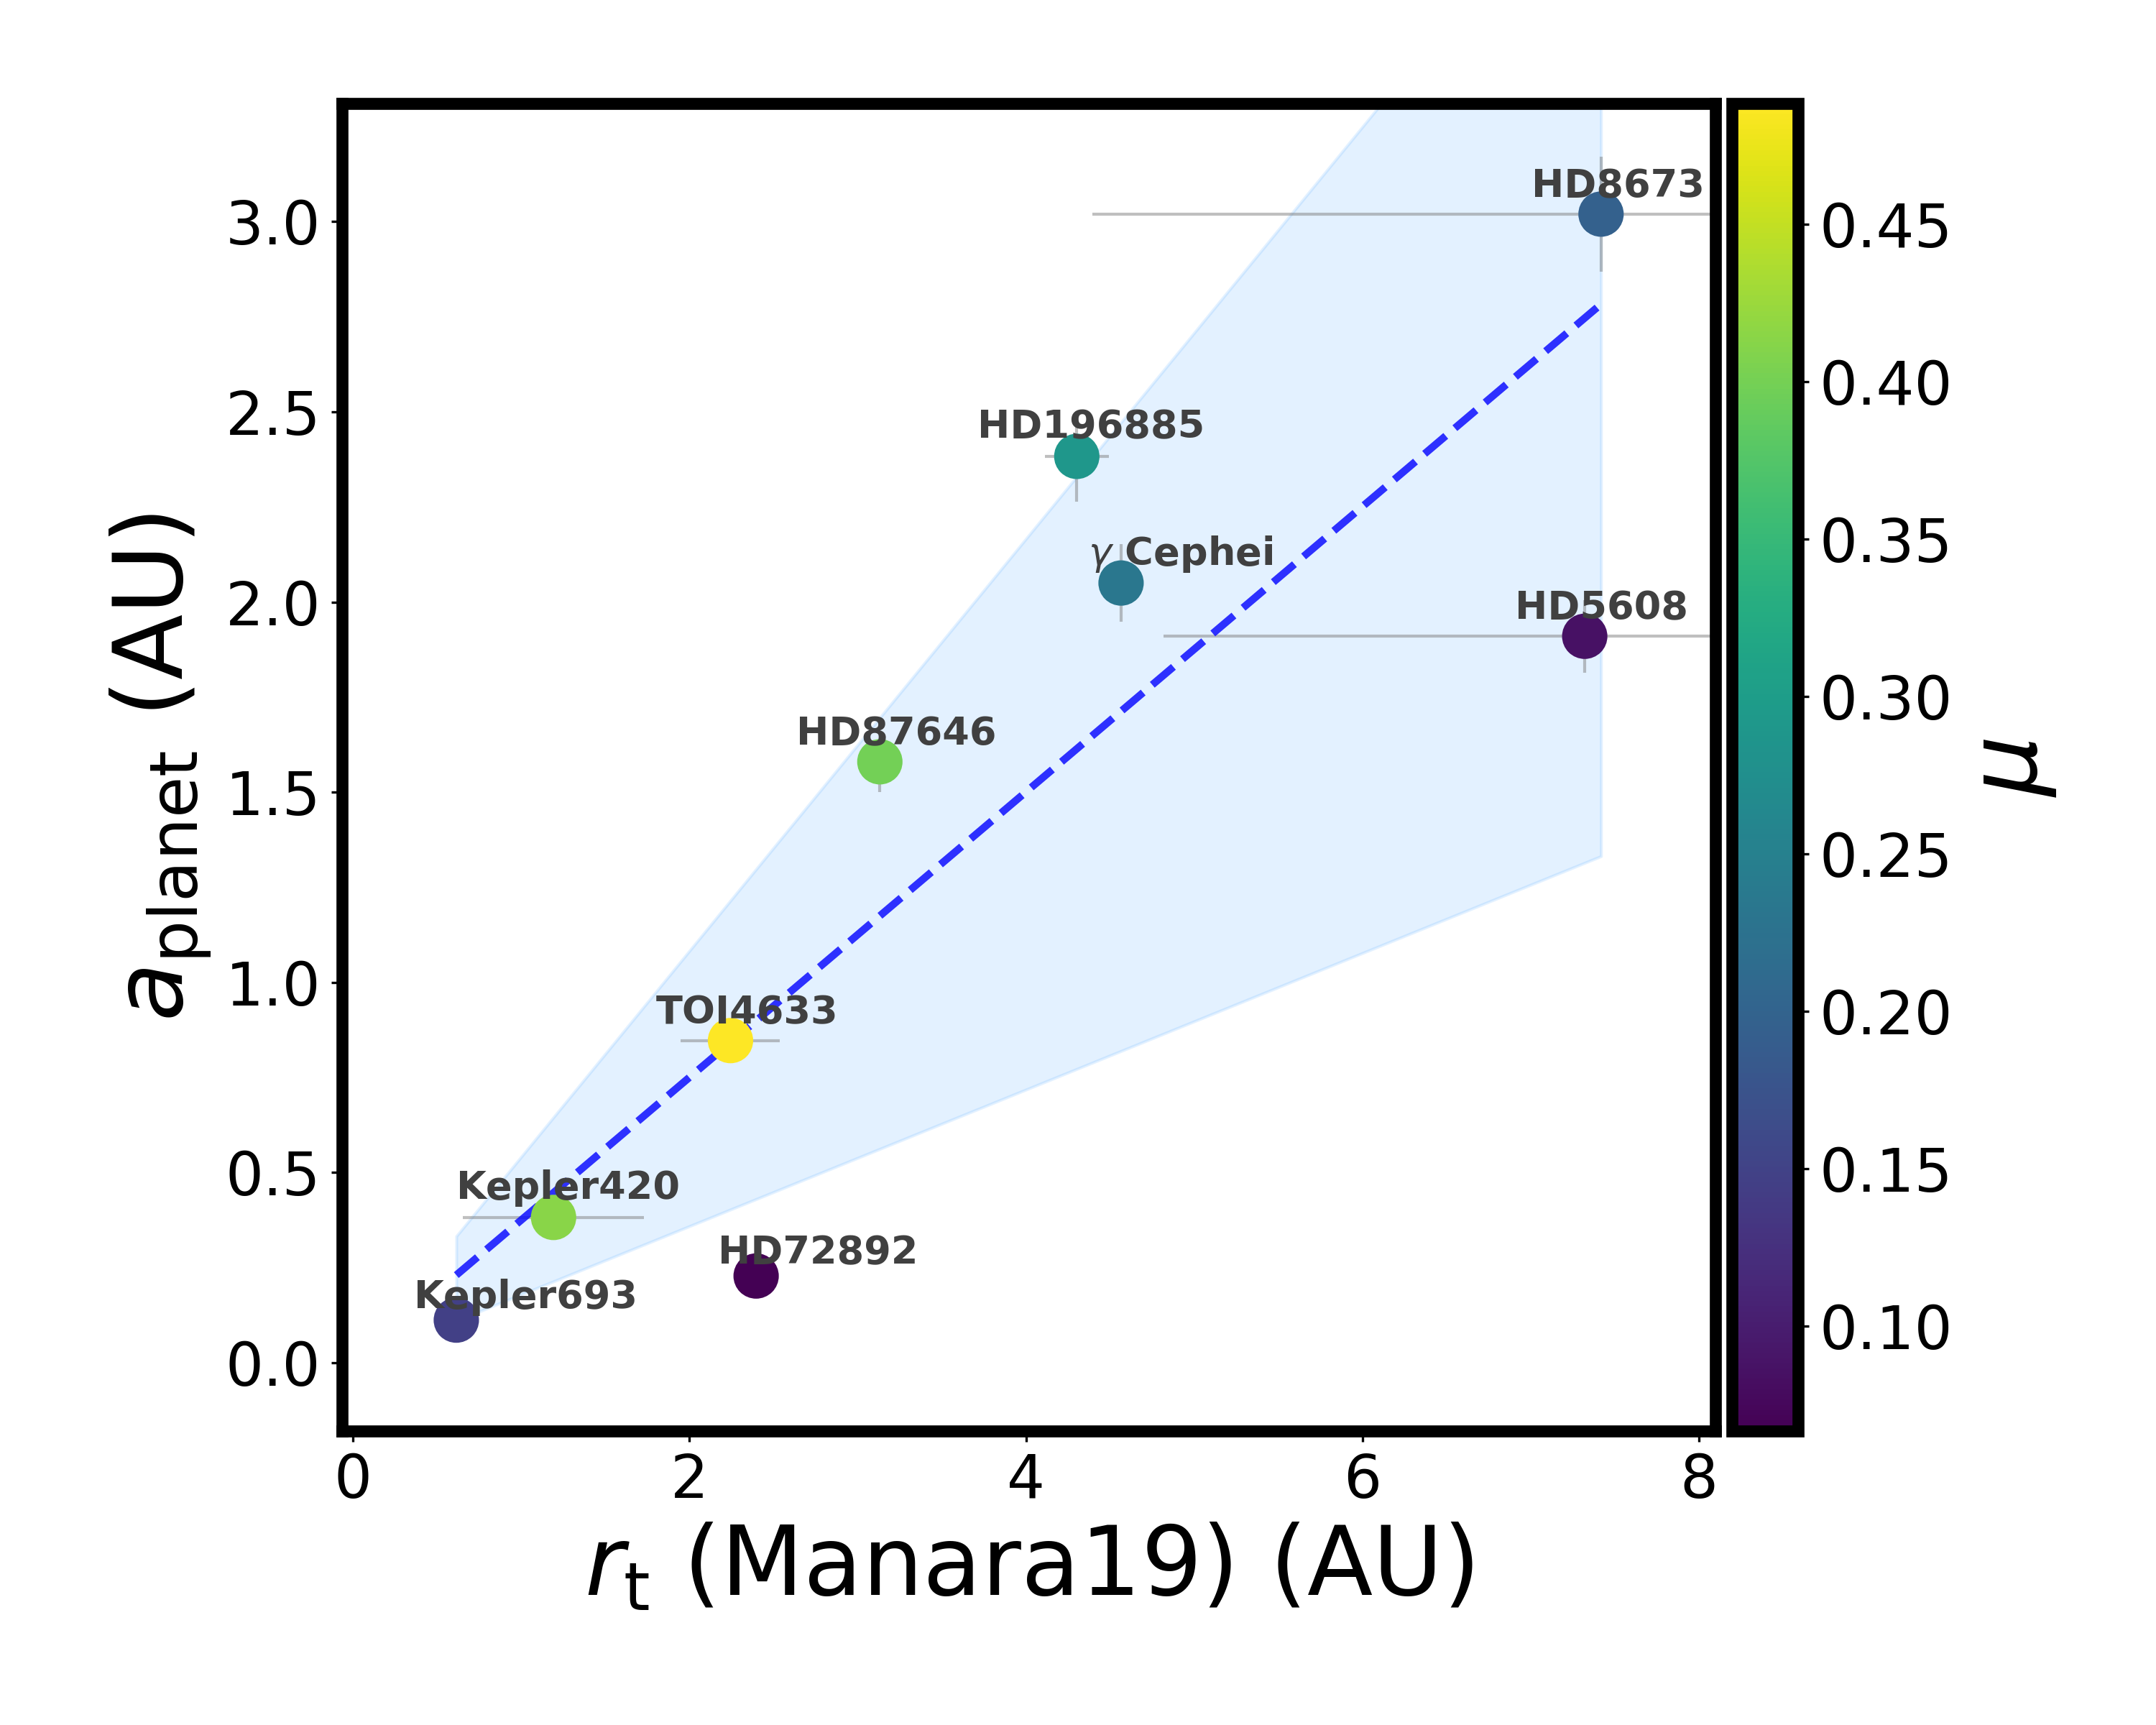
\includegraphics[width=\columnwidth]{scatter_traps_group_unstable_gaints_r_trunc_manara_color_mu_star_all_False.png}
    \caption{Same as Fig.~\ref{fig:trap_vs_observed_goods} but with
    $r_t$ calculated from \rev{Eq.~\eqref{eq:rt_manara}
    \citep{Manara2019A&A...628A..95M}. The dashed line is the fit through
    the origin with slope 0.375; the band is the intrinsic scatter.}}
    \label{fig:rt_manara}
\end{figure}

%% -------------------------------------------------------------------------
\section{Sample parameters}
\label{app:table}

\begin{table*}
\centering
\caption{Stellar and planetary parameters for the sample of unstable gas
giants. Systems marked with $\dagger$ are excluded from the linear-fit
analysis (see Sect.~\ref{sec:results}). \rev{The last column lists the
observed semi-major axis in units of the \citet{Pichardo2005} truncation
radius; `---' indicates that $e_b$ is not measured.}}
\label{tab:stellar_params}
\small
\begin{tabular}{lcccccc}
\hline\hline
System & $m_1\,(M_\odot)$ & $m_2\,(M_\odot)$ & $e_b$ &
$a_b\,(\mathrm{AU})$ & $a_\mathrm{planet}\,(\mathrm{AU})$ & \rev{$a_\mathrm{planet}/r_t$} \\
\hline
$\nu$~Oct$^\dagger$     & $1.57\pm0.06$ & $0.57\pm0.01$  & $0.24\pm0.0003$ & $2.6$          & $1.25$ & \rev{2.12} \\
Kepler~693             & $0.80\pm0.035$& $0.138\pm0.045$& $0.48\pm0.085$  & $2.9\pm0.6$    & $0.112\pm0.0015$ & \rev{0.25} \\
Kepler~420             & $0.99\pm0.05$ & $0.7\pm0.07$   & $0.31\pm0.29$   & $5.3\pm1.3$    & $0.382\pm0.006$ & \rev{0.40} \\
HIP~90988$^\dagger$    & $1.30\pm0.08$ & $0.1\pm0.006$  & $0.29$          & $7.48$         & $1.36$ & \rev{0.75} \\
HD~72892               & $1.02\pm0.05$ & $0.073\pm0.04$ & $0.38\pm0.003$  & $8.124$        & $0.228\pm0.008$ & \rev{0.13} \\
TOI~1736               & $1.08\pm0.04$ & $0.78$         & ---             & $8.2$          & $1.35\pm0.017$ & \rev{---} \\
HD~28192$^\dagger$     & $1.08$        & $0.09\pm0.008$ & $0.029$         & $8.5$          & $0.118$ & \rev{0.04} \\
HD~59686$^\dagger$     & $1.86\pm0.2$  & $0.53\pm0.001$ & $0.729\pm0.004$ & $13.56\pm0.16$ & $1.086$ & \rev{1.19} \\
HD~87646               & $1.12\pm0.09$ & $0.74$         & $0.54$          & $19.5$         & $1.58$ & \rev{0.72} \\
$\gamma$~Cephei        & $1.18$        & $0.36\pm0.022$ & $0.41\pm0.007$  & $19.56\pm0.18$ & $2.05$ & \rev{0.62} \\
HD~196885              & $1.1$         & $0.45\pm0.01$  & $0.42\pm0.02$   & $19.78\pm0.86$ & $2.383$ & \rev{0.75} \\
HD~145934$^\dagger$    & $2.05$        & $0.085\pm0.042$& $0.191\pm0.053$ & $21.774$       & $4.89$ & \rev{0.77} \\
HD~5608                & $1.29\pm0.23$ & $0.12\pm0.008$ & $0.53\pm0.22$   & $30.5$         & $1.91$ & \rev{0.43} \\
HD~8673                & $1.56\pm0.1$  & $0.38\pm0.07$  & $0.5\pm0.25$    & $35$           & $3.02$ & \rev{0.60} \\
HIP~107773             & $2.39\pm0.27$ & $0.63\pm0.04$  & ---             & $40$           & $0.72\pm0.03$ & \rev{---} \\
TOI~4633               & $1.1\pm0.06$  & $1.05\pm0.06$  & $0.91\pm0.03$   & $48.6\pm3.95$  & $0.847$ & \rev{1.17} \\
$\gamma$~Leo$^\dagger$ & $1.41\pm0.14$ & $1.55\pm0.08$  & $0.84$          & $163$          & $1.19$ & \rev{0.25} \\
\hline
\end{tabular}
\end{table*}

\end{appendix}

\end{document}